\begin{abstract}
The same training data can teach a capability to one model and nothing to
another. Curricula and data attribution depend on this effect, but it is unclear
which parts of a model decide what it can learn from given data. We test whether a
circuit that the model learned earlier can be a prerequisite for learning a new
task. We keep the training data fixed, suppress an induction circuit only while the
model trains on a task that uses it, and evaluate every model with the circuit
intact. In a two-layer transformer, suppressing the circuit's previous-token head
during training prevents learning of long-range copying, and supplying the head's
output restores it. Without the circuit, the model learns nothing from the same data
in 600,000 updates. In pretrained Pythia models from 160M to 6.9B parameters,
suppressing induction heads prevents or delays learning of a retrieval task that
uses induction; suppressing control heads does not. With longer training, most
pretrained models learn the task by building a new induction circuit from backup
heads, which attend to the right tokens before training but do not copy them.
Suppressing these heads after training removes the capability, and suppressing them
from the start prevents learning at 410M for 2,000 updates. The delay, 2 to 18 times
the learning time of the controls, depends on how many backup heads remain. Circuits
that a model has already learned can therefore decide whether, and how quickly, it
learns from later data.
\end{abstract}

\section{Introduction}
\label{sec:intro}

Whether a batch of training data teaches a model something new depends on the
model as well as on the data. Curricula, data selection and data attribution all
rely on the fact that the value of an example changes during training
\citep{bengio2009curriculum,chen2023skillit,mindermann2022prioritized,wang2025temporal,lee2026influence},
but it is unclear which part of a model's state decides what the model can learn.
We ask whether a specific learned computation can decide it. If a new capability is
built from computations the model already has, then whether those computations are
available should decide whether the model learns the capability from a given data
stream. We call such computations \emph{prerequisite circuits}.

Testing this idea requires separating two roles a circuit can play. A circuit may be
needed to \emph{perform} a capability, which ablation at evaluation time measures,
or to \emph{learn} it, which such ablation cannot reveal. We isolate the second role
with \emph{training-only suppression}. We zero a circuit's output only on the
training examples of the new task, keep the training batches and their order
identical across conditions, and evaluate every model with the circuit intact
(\figref{fig:rescue}A). Any difference in what the models learn then comes from
whether the circuit was available during training.

Earlier work has intervened on internal structure during training.
\citet{chen2024sudden} suppress syntactic attention while masked language models
train and find it necessary for later grammatical capabilities,
\citet{singh2024needs} clamp parts of a transformer to find what induction heads
need in order to form, and \citet{sahin2025hapax} suppress induction throughout
pretraining. These interventions act on all training data, so they also change how
the structure itself forms. We instead suppress a circuit that has already formed,
only on the new task's examples and with the training data fixed.

\begin{figure}[t]
\centering
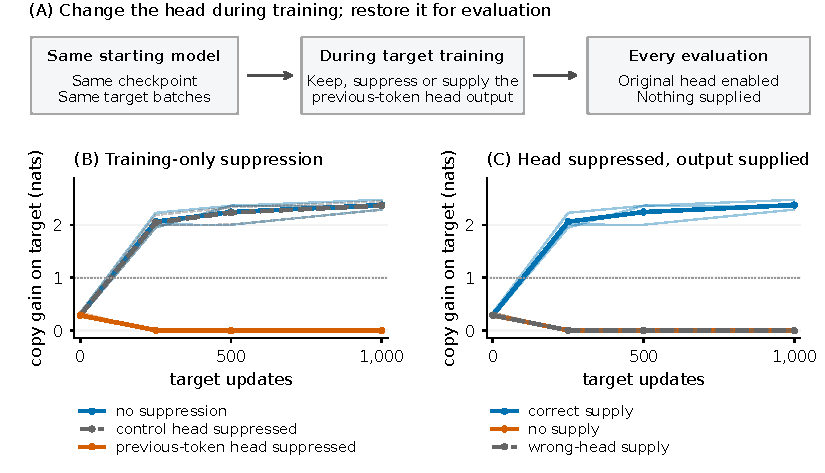
\includegraphics[width=.9\linewidth]{fig_rescue.pdf}
\caption{\textbf{Suppressing the prerequisite during training blocks learning, and
supplying its output restores it} (two-layer model). (A) Every condition starts
from the same checkpoint, trains on the same 1,000 target-task batches and is
evaluated with the original head enabled and nothing supplied. (B) Suppressing the
previous-token head during training blocks learning; suppressing a control head
does not. (C) With the head suppressed, supplying its intact output restores
learning; supplying nothing or the control head's output does not. Thin lines:
three original models; thick lines: means; dotted lines: the 1-nat criterion. Five
further models replicate both results (\appref{app:newseeds}).}
\label{fig:rescue}
\end{figure}

Our prerequisite is induction \citep{olsson2022induction}, in which a
previous-token head and an induction head together predict the token that followed
an earlier occurrence of the current token. Our target tasks build on it. In a
two-layer transformer the target task is long-range copying. In pretrained Pythia
models \citep{biderman2023pythia,vanderwal2025polypythias} it is a retrieval task in
which the model must pass the retrieved token through a fixed mapping. We make three
contributions.

\begin{itemize}[leftmargin=1.2em,itemsep=1pt,topsep=2pt]
\item \textbf{A test of whether learning needs a circuit} (\secref{sec:controlled}).
In the two-layer model, suppressing the previous-token head during training prevents
learning of long-range copying, and supplying the head's output restores it. Data
that do not teach the task before the circuit forms do teach it when replayed
afterwards. Without the circuit, the model learns nothing from the same data in
600,000 updates.
\item \textbf{The same dependence in a pretrained language model}
(\secref{sec:pythia}). In Pythia-160M, suppressing four induction heads on the
target-task examples prevents learning for 500 updates in all 16 public pretraining
runs. Suppressing control heads does not, even when they harm language modeling at
least as much.
\item \textbf{Pretrained models rebuild the prerequisite} (\secref{sec:scaling}).
From 160M to 6.9B parameters, most suppressed models learn the task with longer
training, after 2 to 18 times as many updates as the controls. They turn backup
heads, which attend to the right tokens before training but do not copy them, into
a new induction circuit. Suppressing these heads removes the capability, fewer
remaining backup heads mean a longer delay, and suppressing the new circuit while it
forms prevents the model from learning to retrieve the answer.
\end{itemize}

Our results suggest that a model learns a capability quickly when the circuits it
builds on are present. When they are missing, the model must first rebuild them from
whatever parts it has (\secref{sec:discussion}). The two-layer model cannot rebuild
its previous-token head within our training budgets, whereas pretrained models can
rebuild their induction heads. This rebuilding resembles self-repair by backup heads
\citep{wang2023ioi,mcgrath2023hydra,rushing2024selfrepair} and the relearning of
removed capabilities \citep{lo2024relearn,jain2024mechanistically}. The delay fits
theories in which learning time depends on how many steps must be learned together
\citep{abbe2021staircase,abbe2023leap}.

\section{Setup}
\label{sec:setup}

\paragraph{Prerequisite circuit.}
In a sequence $\ldots A\,B \ldots A$, a first-layer \emph{previous-token head}
writes information about $A$ into the position of $B$. A later \emph{induction head}
attends from the second $A$ to that position and copies $B$
\citep{olsson2022induction}. The previous-token step forms first
\citep{singh2024needs,bietti2023birth,edelman2024evolution}, and the circuit forms
early in pretraining \citep{olsson2022induction,tigges2024consistent}. By the
prerequisite we mean this computation, whichever heads implement it. We call a
head's attention from the repeated token to the token that followed its first
occurrence the head's \emph{induction attention}.

\paragraph{Two-layer model.}
The two-layer model is an attention-only transformer (0.69M parameters, eight heads
per layer, context 128) trained on bytes of enwik8, shuffled to keep bigram
statistics but destroy longer-range structure. \emph{Short repeats} (16-byte spans
copied 17--31 bytes later) form the induction circuit. The target task is
\emph{long repeats} (32-byte spans copied 40--88 bytes later), which reward copying
over a greater distance. We measure learning by \emph{copy gain}: how much lower the
cross-entropy is on copied positions than on the same positions in unmodified text.
A model learns the target task when copy gain reaches 1 nat within 10,000 updates.

\paragraph{Pretrained models.}
We fine-tune public Pythia checkpoints from early in pretraining. We use step 1000
for 160M to 2.8B, where induction has formed, and step 2000 for 6.9B, because its
step-1000 checkpoint falls below our minimum induction accuracy of 0.5. The order
experiments start at step 512 of 160M, before induction forms.

In the target task, \emph{mapped copy}, a four-token key is followed by one of 32
reserved marker tokens, three distractor markers appear elsewhere, and the key
repeats later. The model must output $\pi(m)$, where $m$ is the marker that followed
the key and $\pi$ is a fixed random permutation, so the answer never appears in the
context. Choosing the marker nearest the query scores about 60\% without reading the
key, so we test directly whether the model uses the key. The \emph{key-swap test}
exchanges the key with the tokens before a distractor marker, which changes the
correct answer. The \emph{key-deletion test} replaces the key with unused tokens. We
call a solution \emph{key-dependent} if it passes both tests.

A model \emph{learns} the target task when accuracy reaches 0.8, it passes the
key-swap test on 80\% of pairs and deleting the key lowers accuracy by 0.25 or more.
The 16-run study in \secref{sec:pythia} instead uses an accuracy criterion of 0.5
and runs the key tests at the end of training. Each training batch holds six
mapped-copy examples, six ordinary induction examples and six windows of natural
text.

\paragraph{Interventions.}
\emph{Training-only suppression} zeros the outputs of selected heads on target-task
examples during training. We call the set of suppressed heads the \emph{mask}. In
the pretrained models, the other examples in each batch pass through all heads, all
parameters train and every evaluation removes the mask. In the two-layer model, the
suppressed head and its inputs (embeddings, positions and first normalization) are
frozen in every condition, so the restored head computes exactly the same function.
To test whether the model needs the head's output, we suppress the head and add the
output of an intact frozen copy on the same input. To test the order of training, we
\emph{replay} the same target-task batches in the same order. \emph{Masked
induction} is ordinary induction accuracy measured with the mask applied; it shows
whether the model has rebuilt induction in other heads.

\paragraph{Head selection and controls.}
We never use target-task outcomes to select heads. In the pretrained models we rank
heads by induction attention and suppress the smallest set that lowers held-out
induction accuracy to 0.02 or less (0.2 in the 16-run study). \emph{Matched
controls} are equally many heads in the same layers with the lowest induction
attention. \appref{app:methods} gives details, and \appref{app:hygiene} states which
choices we fixed before which outcomes.

\section{Learning requires the prerequisite in a two-layer model}
\label{sec:controlled}

\paragraph{The circuit is needed during learning.}
We start from three models in which the induction circuit has formed. We identify
the circuit by ablating heads on a short-range copying probe, without reference to
the target task. Ablating the selected heads together lowers short-range accuracy to
0.02 or less; ablating equally many control heads leaves 0.72 or more. We then train
each model for 1,000 updates on long repeats. With no suppression, or with a control
head suppressed, the models learn the target task (copy gain 2.29--2.48 nats). With
the previous-token head suppressed during training, copy gain stays between $-0.03$
and $0.02$ nats (\figref{fig:rescue}B). The head and its inputs are frozen, so the
restored head computes the same function at every evaluation. The conditions
therefore differ only in whether the head's output was available during training.

\paragraph{Supplying the head's output restores learning.}
We keep the head suppressed but add the output of an intact frozen copy. This
restores learning (copy gain 2.29--2.48 nats). Adding nothing, or adding the control
head's output, leaves copy gain below 0.023 nats (\figref{fig:rescue}C). The
supplied output reproduces the intact forward pass to within $2\times10^{-5}$ in the
logits. Five further models, trained from scratch under the same rules, replicate
both results (\appref{app:newseeds}).

\paragraph{The same data teach after the circuit forms.}
We compare two schedules with the same data. One trains on short repeats until the
circuit forms and then on 90,000 target-task batches; the other presents the same
batches first and the short repeats afterwards. After the circuit forms, the batches
yield 2.4 nats or more of copy gain within 10,000 updates. Before it forms, they
yield at most 0.02 nats after all 90,000. A model of the same age trained only on
unmodified text also fails.

We also replay the target-task batches after a first exposure. The first exposure
fails in all three seeds. The circuit then forms in two of them, and in both the
replayed batches teach the target task by the first evaluation at 500 updates. In
the third seed the circuit does not form, and replay fails (\appref{app:controlled},
\figref{fig:orders}). A four-layer transformer with MLP blocks shows the same effect
of order (\appref{app:breadth}).

\paragraph{Without the circuit, the model does not learn.}
Models trained on the target task first stay below 0.03 nats of copy gain for
600,000 updates, 1,200 times the budget that suffices with the circuit. So do models
whose previous-token head we reset after the circuit forms (\appref{app:horizon}).

The two parts of the circuit behave differently. Resetting the previous-token head
(4.8\% of parameters) blocks learning for 90,000 updates in six of six models.
Resetting the selected induction heads instead lets all six learn within 500
updates. After a reset of the whole second layer and the readout, the models do not
recover within 10,000 updates (\appref{app:resets}). In a third group of three
models, the previous-token reset blocks learning in two. The third keeps a second
head with previous-token attention of 0.98 (0.15 or less in every other model), and
resetting that head as well blocks learning (\appref{app:retained}).

In this model, then, the target-task data can rebuild the induction step but not
the previous-token step. In the pretrained models we suppress the induction heads on
target-task examples, so the models cannot rebuild induction in those heads;
\secref{sec:scaling} shows that they rebuild it in other heads.

\section{Learning requires the prerequisite in Pythia-160M}
\label{sec:pythia}

\begin{figure}[t]
\centering
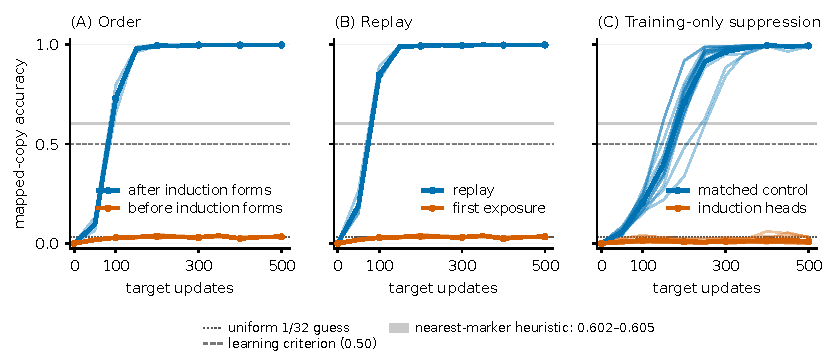
\includegraphics[width=\linewidth]{fig_pythia.pdf}
\caption{\textbf{Order, replay and training-only suppression in Pythia-160M.} Thin
lines average the two data streams of one pretraining run; thick lines average runs
(three in A and B, all 16 in C). (A) Target-task batches arrive after induction
forms (blue) or before (orange). (B) First exposure and replay after induction
forms. (C) Induction heads (orange) or matched control heads (blue) are suppressed
on target-task examples only; every evaluation uses all heads. Dotted and dashed
lines mark uniform guessing and the 0.5 criterion; the band marks the
nearest-marker heuristic.}
\label{fig:pythia}
\end{figure}

\paragraph{Order and replay.}
At pretraining step 512, Pythia-160M cannot yet perform induction: it predicts
none of the 256 repeated tokens on our induction probe. From this checkpoint we
train on the same batches in two orders, in three pretraining runs with two data
streams each. When the model first trains on natural text with synthetic repeats
until induction forms (2,200--2,600 updates) and then on 500 target-task batches,
target accuracy passes 0.5 within 100 updates and ends at 0.99 or above. When the
model trains on the same 500 target-task batches first, accuracy stays at or below
0.066. We then give this model the same induction training. It has now seen
exactly the same batches as the first model, and induction has formed, yet its
target accuracy is still zero. Replaying the 500 target-task batches then brings
accuracy to 0.5 within 100 updates in all six cases (\figref{fig:pythia}A--B).

\paragraph{Training-only suppression in 16 pretraining runs.}
At step 1000 we select four induction heads and suppress them on the mapped-copy
examples only. We use the three original runs and the 13 other public PolyPythias
runs, which vary initialization, data order or both. Target accuracy never exceeds
0.067 on either stream, while every matched control reaches 0.992 or more within 500
updates (\figref{fig:pythia}C; 32 of 32 paired comparisons; one-sided sign test over
runs, $p=2^{-16}$). The controls' solutions are key-dependent: they pass the key-swap
test on 96--100\% of pairs, and deleting the key lowers their accuracy to 2--7\%
(\appref{app:pythia}).

\paragraph{Controls that harm language modeling as much still learn.}
Low-attention heads also matter little for language modeling, so the controls might
learn only because removing them does little damage. We therefore select
\emph{loss-matched controls}. Among heads whose individual removal keeps induction at
90\% of its intact accuracy or more, we add heads in order of how much their removal
raises natural-text loss. We stop when the set raises the loss at least as much as
the induction heads do. At 160M this takes 16 heads, which raise natural-text loss by
0.43 nats (0.40 for the four induction heads) and leave induction at 0.66 (0.00).

Under the protocol of \secref{sec:scaling}, suppressing these 16 heads does not slow
learning: the model learns at updates 350 and 400, against 350 without suppression.
The four induction heads delay learning to 6,300--6,400 updates. At 410M, with eight
loss-matched heads suppressed, the model learns at updates 150 and 200, against 150
without suppression (\appref{app:lossmatched}).

\paragraph{What suppression removes.}
Suppression also changes induction itself: suppressed models end with lower
induction than the controls (0.22--0.49 against 0.74 or more). Blocking only the
target-task gradient through the heads, while keeping their output, does not
reliably prevent learning (\appref{app:gradientblock}). The model therefore needs the
heads' output during training, not a gradient path through them.

\section{Pretrained models rebuild the prerequisite from backup heads}
\label{sec:scaling}

\begin{figure}[t]
\centering
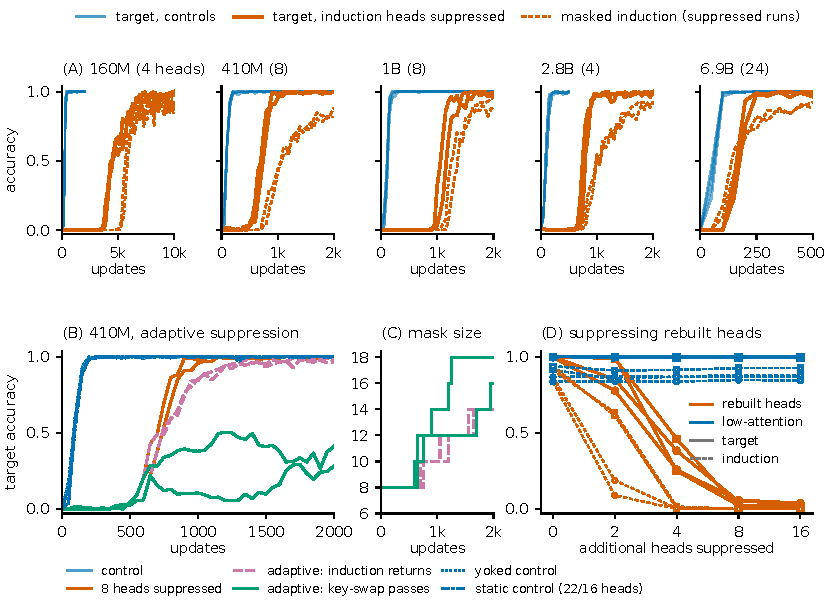
\includegraphics[width=\linewidth]{fig_scaling.pdf}
\caption{\textbf{Pretrained models learn only after rebuilding the prerequisite.}
(A) Target accuracy (solid; evaluated without the mask) and masked induction
(dashed) for suppressed runs (orange) and controls (blue), two data streams per
size; parentheses give the number of suppressed heads. The 2.8B controls come from
the 500-update study, and 6.9B starts at pretraining step 2000. (B) Adaptive
suppression at 410M. Adding heads to the mask whenever masked induction returns
(pink) does not prevent learning. Adding heads whenever the model passes the key-swap
test (green) keeps it from learning a key-dependent solution. Yoked (dotted) and
static (dash-dot) controls with as many low-attention heads suppressed learn by
update 150. (C) Mask size (number of suppressed heads) in the adaptive runs. (D) After training,
suppressing the top rebuilt heads (orange) removes masked induction (dashed) and
target accuracy (solid) at 410M (circles) and 1B (squares); suppressing
low-attention heads in the same layers (blue) does not.}
\label{fig:scaling}
\end{figure}

We repeat training-only suppression at 160M to 6.9B with new data streams, longer
training and a learning rate of $3\times10^{-5}$. We chose this rate on control runs
only, because $10^{-4}$ made control learning unstable at 410M and 1B. At each size
we suppress the smallest set of induction heads, from a coarse grid, that lowers
held-out induction to 0.02 or less (4, 8, 8, 7, 4 and 24 heads). Controls learn
within 100--350 updates at every size. Architecture, head width and checkpoint age
differ across sizes (\appref{app:scaling}), so we treat each size as a separate case
and fit no trend. We did not train 12B, whose step-1000 checkpoint falls below our
induction threshold.

\begin{table}[t]
\centering\small
\caption{\textbf{Training-only suppression across model sizes.} \emph{First learned}
is the first evaluation (every 50 updates) that meets the learning criterion, for
data stream 1 / 2. Masked induction is given at the start and end of training.}
\label{tab:scaling}
\setlength{\tabcolsep}{3.5pt}
\begin{tabular}{@{}lcccccc@{}}
\toprule
Model & Heads & Updates & \multicolumn{2}{c}{First learned} & Delay & Masked induction \\
\cmidrule(lr){4-5}
 & suppressed & observed & controls & suppressed & & start $\to$ end \\
\midrule
160M & 4 & 10,000 & 350 & 6,400 / 6,300 & 18$\times$ & 0.00 $\to$ 0.90 \\
410M & 8 & 2,000 & 150 & 900 / 900 & 6$\times$ & 0.01 $\to$ 0.82--0.88 \\
1B & 8 & 2,000 & 150--200 & 1,200 / 1,400 & 6--9$\times$ & 0.00 $\to$ 0.89--0.96 \\
1.4B & 7 & 500 & 150 & partial$^\dagger$ & --- & 0.01 $\to$ 0.01 \\
2.8B & 4 & 2,000 & 150--200$^\ddagger$ & 900 / 900 & $\approx$5$\times$ & 0.01 $\to$ 0.92--0.93 \\
6.9B$^\ast$ & 24 & 500 & 100 & 200 / 250 & 2--2.5$\times$ & 0.00 $\to$ 0.88--0.92 \\
410M$^\S$ & 8, 4, 4 & 2,000 & 150--200 & 900 / 900; never$^{\times 4}$ & 6$\times$; --- & 0.00 $\to$ 0.82, 0.00 \\
\bottomrule
\end{tabular}\\[2pt]
\raggedright\footnotesize $^\ast$Pretraining step 2000; not comparable to the step-1000 rows. $^\dagger$Target accuracy 0.20 and 0.14 at 500 updates, failing the key tests. $^\ddagger$Controls from the 500-update study on other data streams. $^\S$Three independent pretraining runs (run 1; runs 2 and 3); controls from their 500-update study.
\end{table}

\paragraph{Learning is delayed.}
At 500 updates, the length of the 16-run study, suppression prevents learning at
160M, 410M, 1B and 2.8B and in three independent 410M pretraining runs. With longer
training, the suppressed models learn the target task at every size except 1.4B,
which we train for only 500 updates (\figref{fig:scaling}A; Table~\ref{tab:scaling}).
410M and 1B learn after 900--1,400 updates, 6--9 times as long as the controls. 2.8B
learns after 900 updates. 160M makes no progress for 3,500 updates and learns after
6,300--6,400, 18 times as long as the controls. Of the three independent 410M runs,
one learns at update 900 and two do not learn within 2,000 updates.

\paragraph{The models learn the task before they recover induction.}
Masked induction also recovers, from 0.00 to above 0.8, but only after the target
task. With the mask applied, target accuracy rises before masked induction at 160M,
410M, 1B and 2.8B. At 410M, target accuracy with the mask applied is 0.62 at update
650, while masked induction is 0.004. At 1B it is 0.59--0.63 while masked induction
is zero. Only at 6.9B do the two rise together. The mask applies only to target-task
examples, so only these examples give the models a reason to rebuild induction
outside the suppressed heads. The models first build a retrieval circuit for the
target task itself. Four observations show that this circuit rebuilds the
prerequisite from backup heads.

\paragraph{(a) The target task depends on the rebuilt heads.}
After training, we rank the unsuppressed heads of each model that learned by
induction attention, with the mask applied, and also suppress the top $k$
(\figref{fig:scaling}D). At 410M, suppressing the top four removes held-out
induction (0.84--0.87 to 0.00) and lowers target accuracy from 1.00 to 0.26--0.38;
suppressing eight lowers it to 0.05--0.06. At 1B, four heads lower target accuracy
to 0.25--0.46 and eight to 0.01--0.02. Suppressing equally many low-attention heads
in the same layers changes neither measure. At 6.9B, eleven or twelve more heads
lower induction to 0.01--0.02 and target accuracy to 0.28--0.32
(\appref{app:scaling}).

\paragraph{(b) The rebuilt heads are backup heads.}
In the pretrained 410M and 1B models, these heads rank 9th to 13th by induction
attention, just below the suppressed heads. Before training they already attend from
the repeated key to its source (induction attention 0.11--0.67 with the mask
applied, against a median of 0.01), yet masked induction is 0.00. We call such heads
\emph{backup heads}. Their attention grows during training in every condition,
including the controls. Only suppressed training, however, makes their outputs copy:
masked induction reaches 0.84--0.94 after suppressed training and stays at 0.00
after control or unsuppressed training (\appref{app:regrowth}). The models thus
rebuild the prerequisite from backup heads that were present but unused, much as
backup heads take over from ablated heads at inference
\citep{wang2023ioi,gong2026coax}.

\paragraph{(c) The delay depends on how many backup heads remain.}
If learning waits for backup heads to be repurposed, leaving more of them
unsuppressed should shorten the delay, and suppressing all of them should prevent
learning. We find both effects. At 160M, suppressing only the top two induction
heads still meets our selection criterion (held-out induction 0.012) but leaves three
heads with induction attention above 0.3. The model then learns by update
1,100--1,300. With three heads suppressed it does not learn within 2,000 updates, and
with four it needs 6,300--6,400. At 410M, four suppressed heads permit learning
within 500 updates and eight delay it to 900. At 1B, the same numbers give learning
within 500 updates and at 1,200--1,400.

Conversely, we suppress at 410M every head with induction attention of 0.2 or more
in the pretrained model (13 heads, fixed before training). Target accuracy then stays
at or below 0.012 for all 2,000 updates, while unsuppressed induction and
natural-text loss stay at the levels of the other runs. Suppressing 13 low-attention
heads in the same layers does not slow learning (update 150, as without
suppression). The number of backup heads with induction attention of 0.2 or more
also separates the three independent 410M runs. Run 1 has eight and learns at update
900; runs 2 and 3 have three each and do not learn. We counted the heads of run 3
before training it. Across sizes, the count orders the delays only roughly
(\appref{app:regrowth}).

\paragraph{(d) Suppressing the rebuilt circuit as it forms prevents learning.}
Two adaptive procedures at 410M test whether the models must rebuild the circuit to
learn. Every 50 updates, each procedure computes a score with the mask applied. If
the score exceeds a threshold, the procedure adds to the mask the unsuppressed heads
with the highest attention from the query to the source, until the score falls below
the threshold.

When the score is masked induction (threshold 0.02), the mask grows to 14 and 16
heads and masked induction never exceeds 0.04. The model still learns the target
task, at updates 950 and 1,150 (\figref{fig:scaling}B--C), so suppressing general
induction does not stop the circuit that the model builds for the task. When the
score is the key-swap pass rate on held-out target-task examples (threshold 0.10),
the mask grows to 18 and 16 heads. The model then does not learn the task within
2,000 updates (key-swap accuracy at most 0.23 and 0.09). Target accuracy still rises
to 0.41 and 0.28, but the solution is not key-dependent.

Two controls rule out an effect of suppressing more heads. A yoked control adds
equally many low-attention heads in the same layers at the same updates. A static
control suppresses, from the start, as many low-attention heads as the adaptive runs
end with (22 and 16). Both learn by update 150.

\paragraph{When the circuit cannot be rebuilt in place.}
To test what happens when the layers with the suppressed heads cannot change, we
freeze the embeddings and the lower eight of 16 layers of a 1B model, which contain
the suppressed heads, and suppress those heads on target-task examples
(\appref{app:prefix}). If we instead supply their exact outputs during training, the
model learns as fast as without suppression (at update 300). With the heads
suppressed, learning takes nine times as long (2,750--2,800 updates). The model
learns a key-dependent workaround in its upper layers that works only while the
heads are suppressed: 98\% target accuracy with suppression and 2--4\% without.
Masked induction stays at or below 2/256 throughout, so the workaround does not
perform ordinary induction on our probe, although it may use computations the probe
does not measure.

A stronger intervention removes attention to the earlier key occurrence in every
head. It prevents learning for 2,000 updates at 160M to 1.4B, but it also removes
information the task needs, so we report it only in \appref{app:edges}.

\section{Why a missing prerequisite delays learning}
\label{sec:discussion}

We propose one account of both the block in the two-layer model and the delay in
pretrained models. Suppose a target task combines an existing computation with
something new. When the computation is present, the gradient from target-task
examples only has to build the new part, so the model learns quickly. When the
computation is missing, the data must first build a replacement, which is a harder
learning problem. This account resembles theories in which learning time depends on
the largest \emph{leap}, the number of features that must be learned together
\citep{abbe2021staircase,abbe2023leap}, and results showing that intermediate steps
make otherwise unlearnable tasks learnable \citep{wies2023subtask}. The two-layer
model shows where the difficulty lies. It rebuilds a missing induction step within
500 updates but not a missing previous-token step in 600,000, unless a second
previous-token head survives.

Pretrained models also need the prerequisite, but they obtain it differently. At
410M and 1B, training on the target task turns backup heads that already attend to
the right tokens into induction heads. Leaving more of them unsuppressed shortens
the delay. Suppressing all of them, or suppressing the rebuilt circuit as it forms,
prevents the model from learning a key-dependent solution. This agrees with
self-repair at inference, where other heads or layers partly compensate for ablated
ones \citep{mcgrath2023hydra,rushing2024selfrepair,mcdougall2024copy}, including
otherwise unused backup heads \citep{wang2023ioi,gong2026coax}. It also agrees with
the way circuit roles move between heads during Pythia pretraining
\citep{tigges2024consistent}.

Relearning after removal follows a similar pattern. Pruned concept neurons are
rebuilt elsewhere \citep{lo2024relearn}, unlearned knowledge returns after brief
fine-tuning
\citep{deeb2024unlearning,hu2025jogging,lucki2025adversarial,jain2024mechanistically},
and a 160M model whose induction heads are repeatedly reinitialized grows new ones
\citep{sahin2025hapax}. Our results add that the remaining backup heads decide
whether, and how quickly, the model can learn a new capability that depends on the
removed computation. They also show that the model rebuilds the circuit for the new
task before it recovers the general computation.

It remains open why backup heads can be repurposed. The question mirrors a debate
about why overparameterized networks train well \citep{martinelli2026escape}. On a
lottery-ticket view, training amplifies structure that is already present
\citep{frankle2019lottery}; here that structure is a pretrained head with the right
attention pattern. On an escape-dimension view, extra units turn the plateaus of a smaller network into saddles that gradient descent can leave \citep{fukumizu2000local,simsek2021geometry}.
Our data favor the first view in a narrow form, because we can identify the rebuilt
heads before training. They do not rule out the second: we do not measure the loss
landscape, and in Pythia model size is confounded with architecture and checkpoint
age.

\paragraph{Implications.}
If whether a model learns from data depends on a specific circuit, curricula and
data attribution may benefit from taking the model's circuits into account
\citep{chen2023skillit,lee2026influence,chen2026mda}. Suppressing a capability's
prerequisite is a weak safeguard in pretrained models, because they rebuild it from
spare heads; unlearning and safety fine-tuning are fragile in a similar way
\citep{qi2024finetuning,lee2024mechanistic,che2025tampering,tamirisa2025tamper}.
Finally, a claim that a computation is necessary for learning should state the
training length, because suppression that prevents learning for 500 updates may only
delay it. A probe of the general prerequisite can also miss a circuit that the model
rebuilds for the target task alone.

\section{Related work}
\label{sec:related}

\paragraph{Internal structure and later learning.}
Several studies manipulate internal structure during training and observe later
capabilities. \citet{chen2024sudden} suppress syntactic attention in masked language
models and find it necessary for later grammatical capabilities;
\citet{singh2024needs} clamp subcircuits to identify the sub-computations that
induction formation requires; \citet{zucchet2025facts} supply attention patterns to
bypass a plateau in factual learning; and \citet{feng2025extractive} identify
pretrained structures that let later facts generalize. Pretraining data and
curricula shape which circuits form and how selectively fine-tuning acts
\citep{bruijns2026curricula,chen2026mda,hu2025circuits}, and fine-tuning often
strengthens existing mechanisms \citep{prakash2024finetuning,jain2024mechanistically}.
Ablating a few induction heads in pretrained models sharply impairs pattern-matching
in-context learning \citep{crosbie2025induction}, and \citet{sahin2025hapax} suppress
induction throughout pretraining and find that abstractive in-context learning
survives. Unlike these studies, we start from a circuit the model has already
learned and keep the later training data fixed. We combine training-only
suppression, supplying the suppressed output and replay, evaluate every model
intact, and follow the effect across model sizes and training lengths.

\paragraph{Training history, data influence and interventions.}
Influence functions, data valuation and attribution methods quantify how examples
affect a trained model \citep{koh2017understanding,ghorbani2019data,ilyas2022datamodels,park2023trak},
and recent methods track how influence changes during training
\citep{wang2025temporal,lee2026influence,bae2024source}. Critical periods,
warm-starting and plasticity loss show that training history constrains later
learning \citep{achille2019critical,kleinman2024critical,ash2020warm,dohare2024loss,lyle2023plasticity},
and stagewise development provides internal milestones for such effects
\citep{hoogland2025degeneracy,singh2023transient,reddy2024mechanistic,chan2022data}.
Conclusions from ablation and activation patching depend on the method and metric
\citep{zhang2024patching,heimersheim2024patching,li2024optimal,miller2024faithfulness},
and different-looking circuits can implement the same mechanism
\citep{bayatmakou2026many}. Gradient routing localizes what is learned with
data-dependent gradient masks \citep{cloud2024gradient}; we instead suppress the
forward computation on selected examples while the rest of each batch trains
normally.

\section{Limitations and future work}
\label{sec:limits}

We study one prerequisite, induction, with two copy-based target tasks. The data of
the two-layer model are engineered, and the target task for the pretrained models is
synthetic. We fine-tune early Pythia checkpoints rather than intervene during
pretraining. Architecture, head width, the number of suppressed heads and checkpoint
age vary with model size, and above 160M we mostly have one pretraining run per
size, so we claim no scaling law. Suppressing a head removes everything it computes,
so specificity to induction rests on our controls. Our results depend on the
optimizer, learning rate and training length, and failing the learning criterion
does not imply learning nothing. \appref{app:future} describes further experiments.

\section*{Reproducibility Statement}
Code, experiment configurations, recorded results, and reproduction
instructions are available at
\url{https://github.com/KunwarK13/Prerequisite_Circuits}.
The appendices detail the protocols and per-run results. Matched conditions
use deterministic training streams with verified batch counts and digests.
Pretrained-model experiments start from public Pythia checkpoints.

\section*{AI Use Statement}
We used a language-model assistant for literature retrieval and
discovery, manuscript drafting and editing, synthetic-data generation
code, and assistance with research methodology, implementation,
and interpretation of experimental results. All AI-assisted outputs, code, and analyses were reviewed and verified by the authors. The authors take
responsibility for the final manuscript and all reported results.

\begin{thebibliography}{65}
\providecommand{\natexlab}[1]{#1}
\providecommand{\url}[1]{\texttt{#1}}
\expandafter\ifx\csname urlstyle\endcsname\relax
  \providecommand{\doi}[1]{doi: #1}\else
  \providecommand{\doi}{doi: \begingroup \urlstyle{rm}\Url}\fi

\bibitem[Abbe et~al.(2023)Abbe, Boix-Adsera, and Misiakiewicz]{abbe2023leap}
Emmanuel Abbe, Enric Boix-Adsera, and Theodor Misiakiewicz.
\newblock SGD learning on neural networks: leap complexity and saddle-to-saddle dynamics.
\newblock In \emph{Conference on Learning Theory}, 2023.
\newblock arXiv:2302.11055.

\bibitem[Abbe et~al.(2021)Abbe, Boix-Adsera, Brennan, Bresler, and Nagaraj]{abbe2021staircase}
Emmanuel Abbe, Enric Boix-Adsera, Matthew~S. Brennan, Guy Bresler, and Dheeraj Nagaraj.
\newblock The staircase property: How hierarchical structure can guide deep learning.
\newblock In \emph{Advances in Neural Information Processing Systems}, 2021.
\newblock arXiv:2108.10573.

\bibitem[Achille et~al.(2019)Achille, Rovere, and Soatto]{achille2019critical}
Alessandro Achille, Matteo Rovere, and Stefano Soatto.
\newblock Critical learning periods in deep networks.
\newblock In \emph{International Conference on Learning Representations}, 2019.
\newblock arXiv:1711.08856.

\bibitem[Ash and Adams(2020)]{ash2020warm}
Jordan~T. Ash and Ryan~P. Adams.
\newblock On warm-starting neural network training.
\newblock In \emph{Advances in Neural Information Processing Systems}, 2020.
\newblock arXiv:1910.08475.

\bibitem[Bae et~al.(2024)Bae, Lin, Lorraine, and Grosse]{bae2024source}
Juhan Bae, Wu Lin, Jonathan Lorraine, and Roger Grosse.
\newblock Training data attribution via approximate unrolling.
\newblock In \emph{Advances in Neural Information Processing Systems}, 2024.
\newblock arXiv:2405.12186.

\bibitem[Bayat~Makou et~al.(2026)Bayat~Makou, Niu, Dutta, and Gurevych]{bayatmakou2026many}
Alireza Bayat~Makou, Jingcheng Niu, Subhabrata Dutta, and Iryna Gurevych.
\newblock Many circuits, one mechanism: Input variation and evaluation granularity in circuit discovery.
\newblock \emph{Transactions on Machine Learning Research}, 2026.
\newblock arXiv:2606.06267.

\bibitem[Bengio et~al.(2009)Bengio, Louradour, Collobert, and Weston]{bengio2009curriculum}
Yoshua Bengio, J{\'e}r{\^o}me Louradour, Ronan Collobert, and Jason Weston.
\newblock Curriculum learning.
\newblock In \emph{International Conference on Machine Learning}, pages 41--48, 2009.
\newblock doi: 10.1145/1553374.1553380.

\bibitem[Bhaskar et~al.(2024)Bhaskar, Wettig, Friedman, and Chen]{bhaskar2024edge}
Adithya Bhaskar, Alexander Wettig, Dan Friedman, and Danqi Chen.
\newblock Finding transformer circuits with edge pruning.
\newblock In \emph{Advances in Neural Information Processing Systems}, 2024.
\newblock arXiv:2406.16778.

\bibitem[Biderman et~al.(2023)Biderman, Schoelkopf, Anthony, Bradley, O'Brien,
  Hallahan, Khan, Purohit, Prashanth, Raff, Skowron, Sutawika, and van~der Wal]{biderman2023pythia}
Stella Biderman, Hailey Schoelkopf, Quentin~Gregory Anthony, Herbie Bradley, Kyle
  O'Brien, Eric Hallahan, Mohammad~Aflah Khan, Shivanshu Purohit, USVSN~Sai
  Prashanth, Edward Raff, Aviya Skowron, Lintang Sutawika, and Oskar van~der Wal.
\newblock Pythia: A suite for analyzing large language models across training
  and scaling.
\newblock In \emph{International Conference on Machine Learning}, 2023.
\newblock arXiv:2304.01373.

\bibitem[Bietti et~al.(2023)Bietti, Cabannes, Bouchacourt, Jegou, and Bottou]{bietti2023birth}
Alberto Bietti, Vivien Cabannes, Diane Bouchacourt, Herv{\'e} Jegou, and
  L{\'e}on Bottou.
\newblock Birth of a transformer: A memory viewpoint.
\newblock In \emph{Advances in Neural Information Processing Systems}, 2023.
\newblock arXiv:2306.00802.

\bibitem[Bruijns et~al.(2026)Bruijns, Rubruck, Whitefield, Sandbrink, Barez, and Summerfield]{bruijns2026curricula}
Sebastian~A. Bruijns, Jirko Rubruck, Mia~H. Whitefield, Kai~J. Sandbrink, Fazl Barez, and Christopher Summerfield.
\newblock Pretraining curricula enable selective fine-tuning.
\newblock \emph{arXiv preprint arXiv:2607.04846}, 2026.

\bibitem[Chan et~al.(2022)Chan, Santoro, Lampinen, Wang, Singh, Richemond,
  McClelland, and Hill]{chan2022data}
Stephanie C.~Y. Chan, Adam Santoro, Andrew~K. Lampinen, Jane~X. Wang, Aaditya
  Singh, Pierre~H. Richemond, James~L. McClelland, and Felix Hill.
\newblock Data distributional properties drive emergent in-context learning in
  transformers.
\newblock In \emph{Advances in Neural Information Processing Systems}, 2022.
\newblock arXiv:2205.05055.

\bibitem[Che et~al.(2025)Che, Casper, Kirk, Satheesh, Slocum, McKinney, Gandikota, Ewart, Rosati, Wu, Cai, Chughtai, Gal, Huang, and Hadfield-Menell]{che2025tampering}
Zora Che, Stephen Casper, Robert Kirk, Anirudh Satheesh, Stewart Slocum, Lev~E. McKinney, Rohit Gandikota, Aidan Ewart, Domenic Rosati, Zichu Wu, Zikui Cai, Bilal Chughtai, Yarin Gal, Furong Huang, and Dylan Hadfield-Menell.
\newblock Model tampering attacks enable more rigorous evaluations of LLM capabilities.
\newblock \emph{Transactions on Machine Learning Research}, 2025.
\newblock arXiv:2502.05209.

\bibitem[Chen et~al.(2026)Chen, Luo, and Pan]{chen2026mda}
Jianhui Chen, Yuzhang Luo, and Liangming Pan.
\newblock Mechanistic data attribution: Tracing the training origins of interpretable LLM units.
\newblock In \emph{International Conference on Machine Learning}, 2026.
\newblock arXiv:2601.21996.

\bibitem[Chen et~al.(2023)Chen, Roberts, Bhatia, Wang, Zhang, Sala, and R{\'e}]{chen2023skillit}
Mayee~F. Chen, Nicholas Roberts, Kush Bhatia, Jue Wang, Ce Zhang, Frederic Sala, and Christopher R{\'e}.
\newblock Skill-it! A data-driven skills framework for understanding and training language models.
\newblock In \emph{Advances in Neural Information Processing Systems}, 2023.
\newblock arXiv:2307.14430.

\bibitem[Chen et~al.(2024)Chen, Shwartz-Ziv, Cho, Leavitt, and Saphra]{chen2024sudden}
Angelica Chen, Ravid Shwartz-Ziv, Kyunghyun Cho, Matthew~L. Leavitt, and Naomi Saphra.
\newblock Sudden drops in the loss: Syntax acquisition, phase transitions, and simplicity bias in MLMs.
\newblock In \emph{International Conference on Learning Representations}, 2024.
\newblock arXiv:2309.07311.

\bibitem[Cloud et~al.(2024)Cloud, Goldman-Wetzler, Wybitul, Miller, and Turner]{cloud2024gradient}
Alex Cloud, Jacob Goldman-Wetzler, Ev{\v{z}}en Wybitul, Joseph Miller, and Alexander~Matt Turner.
\newblock Gradient routing: Masking gradients to localize computation in neural networks.
\newblock \emph{arXiv preprint arXiv:2410.04332}, 2024.

\bibitem[Crosbie and Shutova(2025)]{crosbie2025induction}
Joy Crosbie and Ekaterina Shutova.
\newblock Induction heads as an essential mechanism for pattern matching in in-context learning.
\newblock In \emph{Findings of the Association for Computational Linguistics: NAACL 2025}, pages 5049--5111, 2025.
\newblock arXiv:2407.07011.

\bibitem[{\c{S}}im{\c{s}}ek et~al.(2021){\c{S}}im{\c{s}}ek, Ged, Jacot, Spadaro, Hongler, Gerstner, and Brea]{simsek2021geometry}
Berfin {\c{S}}im{\c{s}}ek, Fran{\c{c}}ois Ged, Arthur Jacot, Francesco Spadaro, Cl{\'e}ment Hongler, Wulfram Gerstner, and Johanni Brea.
\newblock Geometry of the loss landscape in overparameterized neural networks: Symmetries and invariances.
\newblock In \emph{International Conference on Machine Learning}, 2021.
\newblock arXiv:2105.12221.

\bibitem[Deeb and Roger(2024)]{deeb2024unlearning}
Aghyad Deeb and Fabien Roger.
\newblock Do unlearning methods remove information from language model weights?
\newblock \emph{arXiv preprint arXiv:2410.08827}, 2024.

\bibitem[Dohare et~al.(2024)Dohare, Hernandez-Garcia, Lan, Rahman, Mahmood, and
  Sutton]{dohare2024loss}
Shibhansh Dohare, J.~Fernando Hernandez-Garcia, Qingfeng Lan, Parash Rahman,
  A.~Rupam Mahmood, and Richard~S. Sutton.
\newblock Loss of plasticity in deep continual learning.
\newblock \emph{Nature}, 632\penalty0 (8026):\penalty0 768--774, 2024.
\newblock doi: 10.1038/s41586-024-07711-7.

\bibitem[Edelman et~al.(2024)Edelman, Tsilivis, Edelman, Malach, and
  Goel]{edelman2024evolution}
Ezra Edelman, Nikolaos Tsilivis, Benjamin~L. Edelman, Eran Malach, and Surbhi
  Goel.
\newblock The evolution of statistical induction heads: In-context learning
  {M}arkov chains.
\newblock In \emph{Advances in Neural Information Processing Systems}, 2024.
\newblock arXiv:2402.11004.

\bibitem[Feng et~al.(2025)Feng, Russell, and Steinhardt]{feng2025extractive}
Jiahai Feng, Stuart Russell, and Jacob Steinhardt.
\newblock Extractive structures learned in pretraining enable generalization on finetuned facts.
\newblock In \emph{International Conference on Machine Learning}, 2025.
\newblock arXiv:2412.04614.

\bibitem[Frankle and Carbin(2019)]{frankle2019lottery}
Jonathan Frankle and Michael Carbin.
\newblock The lottery ticket hypothesis: Finding sparse, trainable neural networks.
\newblock In \emph{International Conference on Learning Representations}, 2019.
\newblock arXiv:1803.03635.

\bibitem[Fukumizu and Amari(2000)]{fukumizu2000local}
Kenji Fukumizu and Shun-ichi Amari.
\newblock Local minima and plateaus in hierarchical structures of multilayer perceptrons.
\newblock \emph{Neural Networks}, 13\penalty0 (3):\penalty0 317--327, 2000.
\newblock doi: 10.1016/S0893-6080(00)00009-5.

\bibitem[Ghorbani and Zou(2019)]{ghorbani2019data}
Amirata Ghorbani and James Zou.
\newblock Data {S}hapley: Equitable valuation of data for machine learning.
\newblock In \emph{International Conference on Machine Learning}, 2019.
\newblock arXiv:1904.02868.

\bibitem[Gong et~al.(2026)Gong, Lu, Wang, Zhang, Wang, Zeng, Xiao, Yuen, and Lim]{gong2026coax}
Zhiren Gong, He Lu, Tiantong Wang, Yichi Zhang, Yixin Wang, Zihao Zeng, Ming Xiao, Chau Yuen, and Wei Yang~Bryan Lim.
\newblock Conditional co-ablation: Recovering self-repair backups in transformer circuits.
\newblock \emph{arXiv preprint arXiv:2607.01940}, 2026.

\bibitem[Hanna et~al.(2024)Hanna, Pezzelle, and Belinkov]{hanna2024faith}
Michael Hanna, Sandro Pezzelle, and Yonatan Belinkov.
\newblock Have faith in faithfulness: Going beyond circuit overlap when finding model mechanisms.
\newblock In \emph{Conference on Language Modeling}, 2024.
\newblock arXiv:2403.17806.

\bibitem[Heimersheim and Nanda(2024)]{heimersheim2024patching}
Stefan Heimersheim and Neel Nanda.
\newblock How to use and interpret activation patching.
\newblock \emph{arXiv preprint arXiv:2404.15255}, 2024.

\bibitem[Hoogland et~al.(2025)Hoogland, Wang, Farrugia-Roberts, Carroll, Wei, and Murfet]{hoogland2025degeneracy}
Jesse Hoogland, George Wang, Matthew Farrugia-Roberts, Liam Carroll, Susan Wei, and Daniel Murfet.
\newblock Loss landscape degeneracy and stagewise development in transformers.
\newblock \emph{Transactions on Machine Learning Research}, 2025.
\newblock arXiv:2402.02364.

\bibitem[Hu et~al.(2025{\natexlab{a}})Hu, Petty, Shi, Merrill, and Linzen]{hu2025circuits}
Michael~Y. Hu, Jackson Petty, Chuan Shi, William Merrill, and Tal Linzen.
\newblock Between circuits and Chomsky: Pre-pretraining on formal languages imparts linguistic biases.
\newblock In \emph{Proceedings of the 63rd Annual Meeting of the Association for Computational Linguistics (Volume 1: Long Papers)}, pages 9691--9709, 2025{\natexlab{a}}.
\newblock arXiv:2502.19249.

\bibitem[Hu et~al.(2025{\natexlab{b}})Hu, Fu, Wu, and Smith]{hu2025jogging}
Shengyuan Hu, Yiwei Fu, Zhiwei~Steven Wu, and Virginia Smith.
\newblock Unlearning or obfuscating? Jogging the memory of unlearned LLMs via benign relearning.
\newblock In \emph{International Conference on Learning Representations}, 2025{\natexlab{b}}.
\newblock arXiv:2406.13356.

\bibitem[Ilyas et~al.(2022)Ilyas, Park, Engstrom, Leclerc, and
  Madry]{ilyas2022datamodels}
Andrew Ilyas, Sung~Min Park, Logan Engstrom, Guillaume Leclerc, and Aleksander
  Madry.
\newblock Datamodels: Understanding predictions with data and data with predictions.
\newblock In \emph{International Conference on Machine Learning}, 2022.
\newblock arXiv:2202.00622.

\bibitem[Jain et~al.(2024)Jain, Kirk, Lubana, Dick, Tanaka, Grefenstette, Rockt{\"a}schel, and Krueger]{jain2024mechanistically}
Samyak Jain, Robert Kirk, Ekdeep~Singh Lubana, Robert~P. Dick, Hidenori Tanaka, Edward Grefenstette, Tim Rockt{\"a}schel, and David Krueger.
\newblock Mechanistically analyzing the effects of fine-tuning on procedurally defined tasks.
\newblock In \emph{International Conference on Learning Representations}, 2024.
\newblock arXiv:2311.12786.

\bibitem[Kamath et~al.(2025)Kamath, Ameisen, Kauvar, Luger, Gurnee, Pearce, Zimmerman, Batson, Conerly, Olah, and Lindsey]{kamath2025tracing}
Harish Kamath, Emmanuel Ameisen, Isaac Kauvar, Rodrigo Luger, Wes Gurnee, Adam Pearce, Sam Zimmerman, Joshua Batson, Thomas Conerly, Chris Olah, and Jack Lindsey.
\newblock Tracing attention computation through feature interactions.
\newblock \emph{Transformer Circuits Thread}, 2025.
\newblock \url{https://transformer-circuits.pub/2025/attention-qk/index.html}.

\bibitem[Kleinman et~al.(2024)Kleinman, Achille, and Soatto]{kleinman2024critical}
Michael Kleinman, Alessandro Achille, and Stefano Soatto.
\newblock Critical learning periods emerge even in deep linear networks.
\newblock In \emph{International Conference on Learning Representations}, 2024.
\newblock arXiv:2308.12221.

\bibitem[Koh and Liang(2017)]{koh2017understanding}
Pang~Wei Koh and Percy Liang.
\newblock Understanding black-box predictions via influence functions.
\newblock In \emph{International Conference on Machine Learning}, 2017.
\newblock arXiv:1703.04730.

\bibitem[Lee et~al.(2024)Lee, Bai, Pres, Wattenberg, Kummerfeld, and Mihalcea]{lee2024mechanistic}
Andrew Lee, Xiaoyan Bai, Itamar Pres, Martin Wattenberg, Jonathan~K. Kummerfeld, and Rada Mihalcea.
\newblock A mechanistic understanding of alignment algorithms: A case study on DPO and toxicity.
\newblock In \emph{International Conference on Machine Learning}, 2024.
\newblock arXiv:2401.01967.

\bibitem[Lee et~al.(2026)Lee, Smith, Adam, and Hoogland]{lee2026influence}
Jin~Hwa Lee, Matthew Smith, Maxwell Adam, and Jesse Hoogland.
\newblock Influence dynamics and stagewise data attribution.
\newblock In \emph{International Conference on Learning Representations}, 2026.
\newblock arXiv:2510.12071.

\bibitem[Li and Janson(2024)]{li2024optimal}
Maximilian Li and Lucas Janson.
\newblock Optimal ablation for interpretability.
\newblock In \emph{Advances in Neural Information Processing Systems}, 2024.
\newblock arXiv:2409.09951.

\bibitem[Lo et~al.(2024)Lo, Barez, and Cohen]{lo2024relearn}
Michelle Lo, Fazl Barez, and Shay~B. Cohen.
\newblock Large language models relearn removed concepts.
\newblock In \emph{Findings of the Association for Computational Linguistics: ACL 2024}, pages 8306--8323, 2024.
\newblock arXiv:2401.01814.

\bibitem[{\L}ucki et~al.(2025){\L}ucki, Wei, Huang, Henderson, Tram{\`e}r, and Rando]{lucki2025adversarial}
Jakub {\L}ucki, Boyi Wei, Yangsibo Huang, Peter Henderson, Florian Tram{\`e}r, and Javier Rando.
\newblock An adversarial perspective on machine unlearning for AI safety.
\newblock \emph{Transactions on Machine Learning Research}, 2025.
\newblock arXiv:2409.18025.

\bibitem[Lyle et~al.(2023)Lyle, Zheng, Nikishin, Avila~Pires, Pascanu, and Dabney]{lyle2023plasticity}
Clare Lyle, Zeyu Zheng, Evgenii Nikishin, Bernardo Avila~Pires, Razvan Pascanu, and Will Dabney.
\newblock Understanding plasticity in neural networks.
\newblock In \emph{International Conference on Machine Learning}, 2023.
\newblock arXiv:2303.01486.

\bibitem[Martinelli et~al.(2026)Martinelli, Brea, and Gerstner]{martinelli2026escape}
Flavio Martinelli, Johanni Brea, and Wulfram Gerstner.
\newblock The puzzling success of overparameterization: Lottery tickets or escape dimensions?
\newblock Preprint, {\'E}cole Polytechnique F{\'e}d{\'e}rale de Lausanne (EPFL Infoscience), 2026.
\newblock doi: 10.5075/epfl.20.500.14299/263577.

\bibitem[McDougall et~al.(2024)McDougall, Conmy, Rushing, McGrath, and Nanda]{mcdougall2024copy}
Callum~Stuart McDougall, Arthur Conmy, Cody Rushing, Thomas McGrath, and Neel Nanda.
\newblock Copy suppression: Comprehensively understanding a motif in language model attention heads.
\newblock In \emph{Proceedings of the 7th BlackboxNLP Workshop: Analyzing and Interpreting Neural Networks for NLP}, pages 337--363, 2024.
\newblock arXiv:2310.04625.

\bibitem[McGrath et~al.(2023)McGrath, Rahtz, Kram{\'a}r, Mikulik, and Legg]{mcgrath2023hydra}
Thomas McGrath, Matthew Rahtz, J{\'a}nos Kram{\'a}r, Vladimir Mikulik, and Shane Legg.
\newblock The Hydra effect: Emergent self-repair in language model computations.
\newblock \emph{arXiv preprint arXiv:2307.15771}, 2023.

\bibitem[Miller et~al.(2024)Miller, Chughtai, and Saunders]{miller2024faithfulness}
Joseph Miller, Bilal Chughtai, and William Saunders.
\newblock Transformer circuit faithfulness metrics are not robust.
\newblock In \emph{Conference on Language Modeling}, 2024.
\newblock arXiv:2407.08734.

\bibitem[Mindermann et~al.(2022)Mindermann, Brauner, Razzak, Sharma, Kirsch,
  Xu, H{\"o}ltgen, Gomez, Morisot, Farquhar, and Gal]{mindermann2022prioritized}
S{\"o}ren Mindermann, Jan~M. Brauner, Muhammed~T. Razzak, Mrinank Sharma,
  Andreas Kirsch, Winnie Xu, Benedikt H{\"o}ltgen, Aidan~N. Gomez, Adrien
  Morisot, Sebastian Farquhar, and Yarin Gal.
\newblock Prioritized training on points that are learnable, worth learning,
  and not yet learnt.
\newblock In \emph{International Conference on Machine Learning}, 2022.
\newblock arXiv:2206.07137.

\bibitem[Olsson et~al.(2022)Olsson, Elhage, Nanda, Joseph, DasSarma, Henighan,
  Mann, Askell, Bai, Chen, Conerly, Drain, Ganguli, Hatfield-Dodds, Hernandez,
  Johnston, Jones, Kernion, Lovitt, Ndousse, Amodei, Brown, Clark, Kaplan,
  McCandlish, and Olah]{olsson2022induction}
Catherine Olsson, Nelson Elhage, Neel Nanda, Nicholas Joseph, Nova DasSarma,
  Tom Henighan, Ben Mann, Amanda Askell, Yuntao Bai, Anna Chen, Tom Conerly,
  Dawn Drain, Deep Ganguli, Zac Hatfield-Dodds, Danny Hernandez, Scott Johnston,
  Andy Jones, Jackson Kernion, Liane Lovitt, Kamal Ndousse, Dario Amodei,
  Tom Brown, Jack Clark, Jared Kaplan, Sam McCandlish, and Chris Olah.
\newblock In-context learning and induction heads.
\newblock \emph{Transformer Circuits Thread}, 2022.
\newblock arXiv:2209.11895.

\bibitem[Park et~al.(2023)Park, Georgiev, Ilyas, Leclerc, and
  Madry]{park2023trak}
Sung~Min Park, Kristian Georgiev, Andrew Ilyas, Guillaume Leclerc, and
  Aleksander Madry.
\newblock {TRAK}: Attributing model behavior at scale.
\newblock In \emph{International Conference on Machine Learning}, 2023.
\newblock arXiv:2303.14186.

\bibitem[Prakash et~al.(2024)Prakash, Rott~Shaham, Haklay, Belinkov, and Bau]{prakash2024finetuning}
Nikhil Prakash, Tamar Rott~Shaham, Tal Haklay, Yonatan Belinkov, and David Bau.
\newblock Fine-tuning enhances existing mechanisms: A case study on entity tracking.
\newblock In \emph{International Conference on Learning Representations}, 2024.
\newblock arXiv:2402.14811.

\bibitem[Qi et~al.(2024)Qi, Zeng, Xie, Chen, Jia, Mittal, and Henderson]{qi2024finetuning}
Xiangyu Qi, Yi Zeng, Tinghao Xie, Pin-Yu Chen, Ruoxi Jia, Prateek Mittal, and Peter Henderson.
\newblock Fine-tuning aligned language models compromises safety, even when users do not intend to!
\newblock In \emph{International Conference on Learning Representations}, 2024.
\newblock arXiv:2310.03693.

\bibitem[Reddy(2024)]{reddy2024mechanistic}
Gautam Reddy.
\newblock The mechanistic basis of data dependence and abrupt learning in an
  in-context classification task.
\newblock In \emph{International Conference on Learning Representations}, 2024.
\newblock arXiv:2312.03002.

\bibitem[Rushing and Nanda(2024)]{rushing2024selfrepair}
Cody Rushing and Neel Nanda.
\newblock Explorations of self-repair in language models.
\newblock In \emph{International Conference on Machine Learning}, 2024.
\newblock arXiv:2402.15390.

\bibitem[Sahin et~al.(2025)Sahin, Feucht, Belfki, Brinkmann, Mueller, Bau, and Wendler]{sahin2025hapax}
Kerem Sahin, Sheridan Feucht, Adam Belfki, Jannik Brinkmann, Aaron Mueller, David Bau, and Chris Wendler.
\newblock In-context learning without copying.
\newblock \emph{arXiv preprint arXiv:2511.05743}, 2025.

\bibitem[Singh et~al.(2023)Singh, Chan, Moskovitz, Grant, Saxe, and Hill]{singh2023transient}
Aaditya~K. Singh, Stephanie C.~Y. Chan, Ted Moskovitz, Erin Grant, Andrew~M. Saxe, and Felix Hill.
\newblock The transient nature of emergent in-context learning in transformers.
\newblock In \emph{Advances in Neural Information Processing Systems}, 2023.
\newblock arXiv:2311.08360.

\bibitem[Singh et~al.(2024)Singh, Moskovitz, Hill, Chan, and
  Saxe]{singh2024needs}
Aaditya~K. Singh, Ted Moskovitz, Felix Hill, Stephanie C.~Y. Chan, and
  Andrew~M. Saxe.
\newblock What needs to go right for an induction head? A mechanistic study of
  in-context learning circuits and their formation.
\newblock In \emph{International Conference on Machine Learning}, 2024.
\newblock arXiv:2404.07129.

\bibitem[Tamirisa et~al.(2025)Tamirisa, Bharathi, Phan, Zhou, Gatti, Suresh, Lin, Wang, Wang, Arel, Zou, Song, Li, Hendrycks, and Mazeika]{tamirisa2025tamper}
Rishub Tamirisa, Bhrugu Bharathi, Long Phan, Andy Zhou, Alice Gatti, Tarun Suresh, Maxwell Lin, Justin Wang, Rowan Wang, Ron Arel, Andy Zou, Dawn Song, Bo Li, Dan Hendrycks, and Mantas Mazeika.
\newblock Tamper-resistant safeguards for open-weight LLMs.
\newblock In \emph{International Conference on Learning Representations}, 2025.
\newblock arXiv:2408.00761.

\bibitem[Tigges et~al.(2024)Tigges, Hanna, Yu, and Biderman]{tigges2024consistent}
Curt Tigges, Michael Hanna, Qinan Yu, and Stella Biderman.
\newblock LLM circuit analyses are consistent across training and scale.
\newblock In \emph{Advances in Neural Information Processing Systems}, 2024.
\newblock arXiv:2407.10827.

\bibitem[van~der Wal et~al.(2025)van~der Wal, Lesci, M{\"u}ller-Eberstein, Saphra, Schoelkopf, Zuidema, and Biderman]{vanderwal2025polypythias}
Oskar van~der Wal, Pietro Lesci, Max M{\"u}ller-Eberstein, Naomi Saphra, Hailey Schoelkopf, Willem Zuidema, and Stella Biderman.
\newblock PolyPythias: Stability and outliers across fifty language model pre-training runs.
\newblock In \emph{International Conference on Learning Representations}, 2025.
\newblock arXiv:2503.09543.

\bibitem[Wang et~al.(2025)Wang, Song, Zou, Mittal, and Jia]{wang2025temporal}
Jiachen~T. Wang, Dawn Song, James Zou, Prateek Mittal, and Ruoxi Jia.
\newblock Capturing the temporal dependence of training data influence.
\newblock In \emph{International Conference on Learning Representations}, 2025.
\newblock arXiv:2412.09538.

\bibitem[Wang et~al.(2023)Wang, Variengien, Conmy, Shlegeris, and Steinhardt]{wang2023ioi}
Kevin Wang, Alexandre Variengien, Arthur Conmy, Buck Shlegeris, and Jacob Steinhardt.
\newblock Interpretability in the wild: a circuit for indirect object identification in GPT-2 small.
\newblock In \emph{International Conference on Learning Representations}, 2023.
\newblock arXiv:2211.00593.

\bibitem[Wies et~al.(2023)Wies, Levine, and Shashua]{wies2023subtask}
Noam Wies, Yoav Levine, and Amnon Shashua.
\newblock Sub-task decomposition enables learning in sequence to sequence tasks.
\newblock In \emph{International Conference on Learning Representations}, 2023.
\newblock arXiv:2204.02892.

\bibitem[Zhang and Nanda(2024)]{zhang2024patching}
Fred Zhang and Neel Nanda.
\newblock Towards best practices of activation patching in language models: Metrics and methods.
\newblock In \emph{International Conference on Learning Representations}, 2024.
\newblock arXiv:2309.16042.

\bibitem[Zucchet et~al.(2025)Zucchet, Bornschein, Chan, Lampinen, Pascanu, and De]{zucchet2025facts}
Nicolas Zucchet, J{\"o}rg Bornschein, Stephanie Chan, Andrew Lampinen, Razvan Pascanu, and Soham De.
\newblock How do language models learn facts? Dynamics, curricula and hallucinations.
\newblock In \emph{Conference on Language Modeling}, 2025.
\newblock arXiv:2503.21676.

\end{thebibliography}


\appendix
\section{Methods}
\label{app:methods}

\subsection{Two-layer model: architecture, data and optimization}
The two-layer model is an attention-only causal transformer with width
256, eight heads per layer, context length 128, pre-layer normalization, and
689,664 trainable parameters. Learned position vectors enter the query and key
streams but not the value stream. Training minimizes next-byte cross-entropy with
batch size 64 and AdamW (learning rate $10^{-3}$, betas $(0.9,0.98)$, weight decay
0.1, 200 warm-up updates). Every condition begins with the same 2,000-update
warm-up on unmodified text for its seed.

All corpora derive from one 100\,MB order-2 Eulerian shuffle of enwik8, which
preserves byte-bigram counts but destroys longer-range structure. The base corpus
is this shuffle. The short-repeat corpus copies 16-byte spans forward by a
uniformly sampled distance in 17--31 at 400,000 seeded sites. The long-repeat
(target) corpus copies 32-byte spans forward by a distance in 40--88 at 170,000
sites. Training crops start below byte 90M; held-out evaluations start at byte
95M. Each corpus has its own deterministic crop-position generator, so moving a
block of training in time changes when a batch is seen but not which batches are
seen or in what order. Replay rewinds only the target generator. Every
result record stores source counts, generator state, corpus hashes and a digest
of all crop positions, and the scorers reject any mismatch.

\emph{Copy gain} (\texttt{uptake} in the implementation code) is
$\mathrm{CE}_{\text{base}}(\theta;M)-\mathrm{CE}_{\text{target}}(\theta;M)$, where both
cross-entropies are computed at the positions $M$ inside pasted spans, on paired
crops of the unmodified and target corpora. The key probe presents a four-byte key
twice and asks for the byte that followed its first occurrence, at distances 24,
64 and 96 (256 examples each, drawn from the 96 most frequent bytes and generated
independently of the training data). Unless stated otherwise, we evaluate every
500 updates, and endpoint values average the final five evaluations.

\paragraph{Formation rule and schedules.}
After the shared warm-up, the \emph{prerequisite-first} schedule trains on short
repeats until two consecutive distance-24 probe evaluations are at least 0.70, no
earlier than update 10,000 and with a 120,000-update cap, then trains on 90,000
target batches. The \emph{target-first} schedule consumes the same 90,000 target
batches first, then exactly as many short-repeat batches as its paired
prerequisite-first run used (Table~\ref{tab:g1core}).

\begin{table}[!htbp]
\centering\small
\caption{Order comparison with fixed data in the two-layer model. Copy gain is the
maximum in the first 10,000 target updates; the endpoint averages the last five
evaluations. \emph{Data match} requires equal target batch counts and position
digests within each seed.}
\label{tab:g1core}
\begin{tabular}{lrrrrrl}\toprule
 & & \multicolumn{2}{c}{prerequisite first} & \multicolumn{2}{c}{target first} & \\
\cmidrule(lr){3-4}\cmidrule(lr){5-6}
seed & formation update & copy gain $\le$10k & end $d{=}64$ & copy gain $\le$10k & end $d{=}64$ & data match\\\midrule
531 & 59,500 & 2.57 & 0.52 & 0.00 & 0.01 & yes \\
532 & 40,000 & 2.40 & 0.52 & 0.03 & 0.00 & yes \\
533 & 84,000 & 2.58 & 0.61 & -0.03 & 0.01 & yes \\
\bottomrule\end{tabular}
\end{table}

\subsection{Two-layer model: circuit identification and interventions}
\label{app:interventions}
In each model in which the prerequisite has formed, we zero each head's output in
turn. The circuit is every head whose individual removal lowers distance-24
accuracy by at least 45\% of its intact value, capped at four per layer. Controls are equally many
heads with at most a 15\% drop, matched by layer where possible (one control in
seed 532 comes from the other layer). We set this rule after seeing the first
two identification tables and applied it unchanged to the third seed and to all
later seeds. Table~\ref{tab:circuits} gives the selected heads and manipulation
checks.

\emph{Reset} redraws a head's query, key, value, and output weights from the
model's original initialization distribution with a recorded seed; the model then
receives a fresh AdamW optimizer and the first 90,000 batches of the same target
stream. The conditions are \emph{no edit}; \emph{control reset}; \emph{circuit
reset} (all selected heads); \emph{age-matched control} (the warm-up state after an
equal number of additional base-corpus updates); \emph{previous-token reset} (the
largest-effect first-layer head only); \emph{induction-head reset} (every selected
second-layer head); and \emph{heads frozen} (the weights of the six selected heads
are fixed, but gradients still pass through them).

\begin{table}[!htbp]
\centering\small
\caption{Per-seed circuit identification. Heads are layer.head. The
joint-ablation columns report distance-24 accuracy after zeroing the circuit or the
controls.}
\label{tab:circuits}
\resizebox{\linewidth}{!}{%
\begin{tabular}{lrlrlr}\toprule
seed & intact $d{=}24$ & circuit heads & joint ablation & control heads & joint ablation\\\midrule
531 & 0.73 & 1.2, 1.7, 1.0, 2.7, 2.3, 2.6 & 0.012 & 1.1, 1.4, 1.6, 2.5, 2.2, 2.0 & 0.72 \\
532 & 0.72 & 1.3, 1.2, 1.7, 1.5, 2.6, 2.0 & 0.004 & 1.6, 1.4, 1.0, 2.1, 2.3, 2.2 & 0.81 \\
533 & 0.73 & 1.5, 1.6, 1.0, 2.6, 2.5, 2.4 & 0.020 & 1.3, 1.7, 1.4, 2.0, 2.2, 2.3 & 0.82 \\
\bottomrule\end{tabular}}
\end{table}

\paragraph{Training-only suppression with exact restoration.}
Each model uses its previous-token head (the largest-effect first-layer head) and a
low-effect first-layer control head, chosen from the identification records by the
smallest absolute change in base-text loss. We freeze the query, key and value rows
and output columns of both heads, the token embeddings, the positions and the first
normalization. The two heads receive the same first-layer inputs, so this fixes
their complete input path (164,352 parameters). Everything else trains.

The unsuppressed, control-suppressed and suppressed conditions receive the first
1,000 target batches. A fourth condition suppresses the previous-token head while
training on unmodified text at the same crop positions. Every evaluation enables
both heads.

To supply the head's output, we use the same models and freezing. We suppress the
previous-token head's own output in every training forward pass and add one of
three signals to the first-layer attention output: the head's intact contribution,
computed by a frozen copy of the starting model on the same tokens; the control
head's contribution; or nothing. Supplied activations are detached. We do not rescale
the wrong-head supply, so activation norms are not matched. Every evaluation
disables both suppression and supply. The correct supply reproduces the
unsuppressed forward pass to within $2.1\times10^{-5}$ in the logits on fixed audit
sequences.

\subsection{Pretrained models}
\label{app:pythiamethods}
\paragraph{Batches and optimization.}
One optimizer update uses 18 sequences of length 128, in micro-batches of six,
with AdamW (betas $(0.9,0.95)$, weight decay 0.01, gradient-norm clipping at 1) in
FP32. The original 160M studies use learning rate $10^{-4}$ and 500 updates. The
scaling studies use $3\times10^{-5}$. We chose this rate by a search over
$\{3\times10^{-5},10^{-5},3\times10^{-6}\}$ that used only unsuppressed and control
runs on separate development streams; it is the first rate in the search at which
every control learned. In the order and replay study, the induction-forming batch
contains six natural-text windows with six copied six-token spans, six random-token
sequences with six copied spans and six untouched natural windows (copy distances
24--64).

\paragraph{Target batches and probes.}
A target batch contains six mapped-copy sequences, six ordinary induction
sequences (random tokens with a four-token key repeated 24--64 tokens later) and
six natural-text windows. In mapped copy, the token after the first key is one of
32 reserved markers, three distractor markers make the source ambiguous, and the
correct continuation of the repeated key is the marker's image under a fixed random
involution. Accuracy is the full-vocabulary argmax at the query position.

Probes contain 256 held-out sequences, and natural-text loss uses 64 held-out
windows. Each target-stream seed determines both the data and the involution. The
scaling studies use a corrected version of the ordinary-induction training rows, in
which the token after the repeated key is the copied continuation; in the original
implementation it was random. The correction changes no qualitative outcome at 160M, 410M
or 1B (\appref{app:scaling}).

\paragraph{Head selection.}
On an ordinary induction probe (seed 1701), we record each head's attention from
the query (the last token of the repeated key) to the source (the token after the
key's first occurrence). Circuit sets are the top-$k$ heads for increasing $k$.
Controls take, in each layer of the circuit set, the lowest-attention head not
already chosen. We select the smallest $k$ for which, on two calibration probes,
suppressing the circuit leaves induction accuracy at most 0.02 (0.2 in the
original 160M study) with a drop of at least 0.3, while the controls retain at
least 0.5 with a drop of at most 0.15. A new 1,024-example probe verifies the
choice. Where the lowest-attention controls remove too much induction (1.4B, 6.9B
and 12B), we search for layer-matched controls among heads in the lower half of
attention scores. Table~\ref{tab:selection} lists the selections.

\paragraph{Key-dependence tests.}
The \emph{key-swap} test exchanges the true source's four-token key with the four
tokens before a different-valued distractor in the legal window. This keeps the
query, all marker identities and positions, and the multiset of tokens fixed, but
changes the correct answer, so no rule that uses only marker identities and
positions can answer both versions. Eligible pairs are determined without model
outcomes (typically 130--150 of 256 examples). The \emph{key-deletion} test
replaces the true key with unused tokens. The nearest-marker heuristic scores
60.2--60.5\%.

\section{What was fixed in advance}
\label{app:hygiene}
Head selections use only induction probes, never target outcomes, and we choose
learning rates on control and unsuppressed runs only. We wrote down the learning
criteria, training lengths and evaluation schedules before the corresponding target runs.
We report every planned model, seed and pretraining run, including failures. We
calibrated the head-selection threshold of the two-layer model on the first two
seeds and applied it unchanged thereafter.

In the two-layer model the replication unit is the initialization and data seed.
In Pythia it is the public pretraining run, and the two target streams within a run
are technical replicates.

Several analyses are post hoc, and we label them as such where they appear: the
timing analysis of delayed learning (\secref{sec:scaling}), the per-head attention
analyses (\appref{app:regrowth}) and the initial-score comparison in
\appref{app:resets}. We designed the adaptive-suppression, loss-matched-control,
longer-training and additional-seed experiments after the main scaling results
were known, but fixed their rules before their own outcomes. Interrupted runs
resume from saved model, optimizer and data-stream state, and we checked that the
overlapping evaluations match exactly.

The follow-up experiments added for this version have the following history. A
first key-triggered variant used plain target accuracy under the mask (threshold
0.10) as its score. That score sits near its noise floor from the start
(0.05--0.10 before any key-dependent learning), so it triggered on noise. We stopped
those runs at update 400--500 and replaced the score with the key-swap pass rate
before any key-triggered outcome was known; we do not report the stopped runs.

The first 2.8B launch ran out of GPU memory at update 0, and we restarted it from
scratch. We stopped the 160M loss-matched runs at update 600 to free memory and
reran them from scratch with identical settings; the rerun matches the stopped run
at every shared evaluation. We paused one independent 410M run (process suspended)
and resumed it without changing its state. We designed the adaptive procedures, the
13-head mask rule, the static and yoked controls, the loss-matched selection and the
160M dose runs after seeing that models with fixed masks eventually learn, but fixed
their rules before their own outcomes.

\section{Complete results for the two-layer model}
\label{app:controlled}

\begin{figure}[!htbp]
\centering
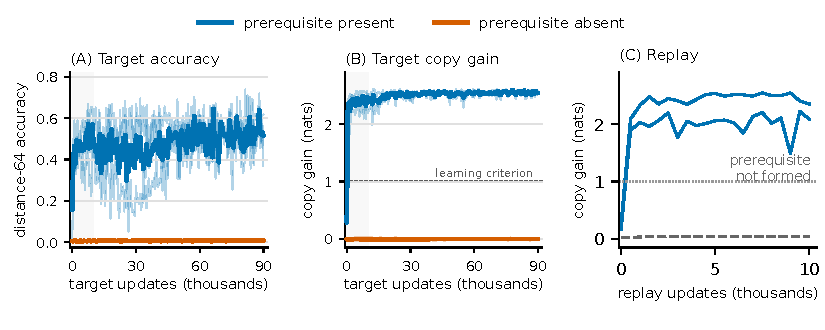
\includegraphics[width=\linewidth]{fig_orders.pdf}
\caption{\textbf{The same data teach only after the prerequisite forms}
(two-layer model). (A--B) Within each seed, both schedules receive the same
90,000 target batches in the same order, either after the induction circuit forms
(blue) or before it (orange). Thin lines are three seeds and thick lines are means;
the shaded region is the 10,000-update learning window. (C) Replay: the
model sees the target stream, then short repeats, then the identical target stream
again. The two models in which the circuit formed learn on replay; the model in
which it did not form (gray) does not.}
\label{fig:orders}
\end{figure}

\begin{table}[!htbp]
\centering\small
\caption{Outcomes of all circuit interventions in the three original models.
Start accuracy is measured immediately after the edit. \emph{First $\ge$1 nat} is
the first evaluation that crosses the criterion; \emph{none} means no crossing in
90,000 updates.}
\label{tab:c1core}
\resizebox{.94\linewidth}{!}{%
\begin{tabular}{llrrrrl}\toprule
seed & intervention & start $d{=}24$ & copy gain $\le$10k & first $\ge$1 nat & end $d{=}64$ & outcome\\\midrule
531 & No edit & 0.73 & 2.56 & 500 & 0.47 & learned \\
531 & Control reset & 0.70 & 2.53 & 500 & 0.61 & learned \\
531 & Circuit reset & 0.01 & 0.00 & none & 0.01 & not learned \\
531 & Age-matched control & 0.01 & 0.00 & none & 0.01 & not learned \\
531 & Previous-token reset & 0.01 & 0.00 & none & 0.01 & not learned \\
531 & Induction-head reset & 0.02 & 2.46 & 500 & 0.32 & learned \\
531 & Heads frozen & 0.73 & 2.50 & 500 & 0.60 & learned \\
532 & No edit & 0.72 & 2.40 & 500 & 0.50 & learned \\
532 & Control reset & 0.82 & 2.38 & 500 & 0.69 & learned \\
532 & Circuit reset & 0.01 & 0.02 & none & 0.00 & not learned \\
532 & Age-matched control & 0.01 & 0.02 & none & 0.00 & not learned \\
532 & Previous-token reset & 0.01 & 0.02 & none & 0.00 & not learned \\
532 & Induction-head reset & 0.03 & 2.39 & 500 & 0.59 & learned \\
532 & Heads frozen & 0.72 & 2.40 & 500 & 0.77 & learned \\
533 & No edit & 0.73 & 2.58 & 500 & 0.63 & learned \\
533 & Control reset & 0.76 & 2.59 & 500 & 0.63 & learned \\
533 & Circuit reset & 0.02 & -0.03 & none & 0.01 & not learned \\
533 & Age-matched control & 0.01 & -0.03 & none & 0.01 & not learned \\
533 & Previous-token reset & 0.02 & -0.02 & none & 0.01 & not learned \\
533 & Induction-head reset & 0.04 & 2.57 & 500 & 0.60 & learned \\
533 & Heads frozen & 0.73 & 2.56 & 500 & 0.62 & learned \\
\bottomrule\end{tabular}}
\end{table}

\begin{table}[!htbp]
\centering\small
\caption{Replay within one model. Copy gain columns are maxima over the full
first exposure and the first 10,000 replay updates. \emph{Exact} verifies that the
generator was rewound and that both presentations used the same 90,000 batches in
the same order.}
\label{tab:replay}
\begin{tabular}{llrrrrl}\toprule
seed & circuit formed & first exposure & replay $\le$10k & first $\ge$1 nat & replay end $d{=}64$ & exact\\\midrule
531 & yes & 0.00 & 2.22 & 500 & 0.55 & yes \\
532 & no (cap) & 0.03 & 0.05 & -- & 0.00 & yes \\
533 & yes & -0.02 & 2.55 & 500 & 0.75 & yes \\
\bottomrule\end{tabular}
\end{table}

\paragraph{Training-only suppression and replay afterwards.}
Table~\ref{tab:stable} reports every endpoint of the suppression experiment. After
the suppressed exposure, the suppressed and unmodified-text conditions receive
exact target replay with both heads enabled and fresh optimizers. No model learns
immediately when the suppressed head is re-enabled.

Replay afterwards gives mixed results. In seed 531 the model learns after
suppressed target exposure but not after unmodified-text exposure, which is
compatible with a latent benefit from the suppressed exposure. Seed 532 learns in
neither case, and seed 533 learns in both. Re-enabling a head therefore guarantees
neither that the heads reading its output remain compatible nor that replay
recovers within 1,000 updates.

\begin{table}[htbp]\centering\small
\caption{Training-only suppression and subsequent replay (copy gain in nats, both
heads enabled). Each phase lasts 1,000 updates. The last two columns start from the
suppressed-target and unmodified-text endpoints.}\label{tab:stable}
\begin{tabular}{lllllll}\toprule
seed & unsuppressed & control & suppressed & unmodified text & replay & text + target \\
\midrule
531 & 2.366 & 2.368 & -0.002 & -0.005 & 1.546 & 0.008 \\
532 & 2.295 & 2.292 & 0.022 & 0.021 & 0.032 & 0.028 \\
533 & 2.481 & 2.453 & -0.029 & -0.034 & 2.366 & 2.332 \\
\bottomrule\end{tabular}
\end{table}

\begin{table}[htbp]\centering\small
\caption{Supplying the head's output, evaluated with the intact head. Entries are copy gain
(nats) / distance-64 accuracy after 1,000 updates.}\label{tab:supply}
\begin{tabular}{llll}\toprule
seed & correct supply & no supply & wrong-head supply \\
\midrule
531 & 2.366 / 0.438 & -0.002 / 0.012 & -0.002 / 0.012 \\
532 & 2.295 / 0.336 & 0.022 / 0.004 & 0.022 / 0.004 \\
533 & 2.481 / 0.340 & -0.029 / 0.008 & -0.030 / 0.008 \\
\bottomrule\end{tabular}
\end{table}

\paragraph{Additional seeds.}
Five further seeds, trained from scratch under the same rules, replicate both the
suppression result and the result of supplying the head's output
(\appref{app:newseeds}).

\paragraph{Transfer and restricted plasticity.}
We transfer the six selected heads, together with the token embeddings, positions,
readout and all normalizations, from a model in which the prerequisite has formed
into its own earlier (warm-up) checkpoint. The transferred model learns the target
task; transferring six control heads with the same interface does not help
(Table~\ref{tab:transfer}). The transfer changes 52.5\% of parameters, and neither
the heads alone nor the heads with positions install the prerequisite. The result
therefore shows transfer of learned weights, not a minimal circuit transplant.

Holding the weights of the selected heads fixed still permits 1.86--2.36 nats of
copy gain by 500 updates, and training only those heads also yields copy gain. The
adaptation that follows the circuit therefore has no unique location.

\begin{table}[htbp]\centering\small
\caption{Transfer and restricted plasticity (copy gain in nats; the maximum
excludes update zero; endpoint accuracy averages the last five
evaluations).}\label{tab:transfer}
\begin{tabular}{lllll}\toprule
seed & intervention & initial & max $\le$10k & end $d{=}64$ \\
\midrule
531 & Circuit transfer & 0.142 & 2.533 & 0.594 \\
531 & Control transfer & -0.001 & -0.003 & 0.014 \\
531 & Only heads train & 0.259 & 2.503 & 0.105 \\
532 & Circuit transfer & 0.289 & 2.388 & 0.634 \\
532 & Control transfer & 0.017 & 0.024 & 0.003 \\
532 & Only heads train & 0.266 & 2.417 & 0.579 \\
533 & Circuit transfer & 0.390 & 2.526 & 0.524 \\
533 & Control transfer & -0.042 & -0.030 & 0.007 \\
533 & Only heads train & 0.337 & 2.534 & 0.478 \\
\bottomrule\end{tabular}
\end{table}

\section{Resetting the previous-token head or the induction heads}
\label{app:resets}

\begin{figure}[htbp]
\centering
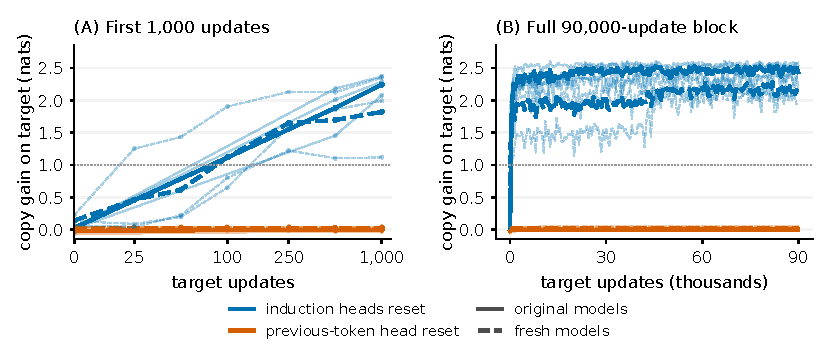
\includegraphics[width=\linewidth]{fig_hero.pdf}
\caption{\textbf{Resetting the previous-token head blocks learning; resetting the
induction heads does not.} All parameters train on the same target stream after
either the largest-effect first-layer (previous-token) head is reset (orange) or the
selected second-layer (induction) heads are reset (blue). (A) First 1,000 updates
(axis linear to 25 updates, logarithmic after). (B) The full 90,000 updates. Thin
lines are three original (solid) and three fresh (dashed) models; thick lines are
means.}
\label{fig:hero}
\end{figure}

Resetting the previous-token head changes 4.8\% of the parameters and changes
base-text loss by at most 0.01 nats relative to no edit. In the three original
models and three fresh models (seeds 1541--1543, run under the same pre-specified
rules), it blocks learning throughout 90,000 target updates. Resetting the selected
second-layer (induction) heads instead lets all six models learn within 500 updates
(\figref{fig:hero}). Control resets preserve learning.

Both resets reduce initial short-range accuracy to at most 0.036 in the original
models. In the fresh models, however, a pre-specified test of equal initial
impairment on the target failed (Table~\ref{tab:mfc_initial}): after the
induction-head reset the models start slightly better on the target (by 1--8
percentage points of distance-64 accuracy and 0.07--0.23 nats of loss). The
comparison therefore shows a difference in recovery between two specific lesions,
not between equally impaired models.

A second group of fresh models (seeds 2641--2643) resets \emph{all} eight second-layer heads
and the output readout. This broader lesion starts no better than the previous-token
reset on either target measure and does not recover within 10,000 updates
(Tables~\ref{tab:dominanceinitial}--\ref{tab:dominancerecovery}). Damage to the
second layer is thus not always easy to repair: within this budget the model
rebuilds the selected induction heads but not the whole second layer and readout.
In the same group the previous-token reset blocks learning in two models and allows
it (at update 3,000) in the third, which \appref{app:retained} explains.

\begin{table}[!htbp]
\centering\small
\caption{Pre-specified initial matching in the fresh reset models. P and S denote
the previous-token reset and the reset of the selected second-layer heads; correct
counts are out of 4,096 per condition. Intervals use a simultaneous 0.05 error
allocation. Matching requires the accuracy interval within $\pm2$ percentage points,
the loss interval within $\pm0.1$ nats and both accuracy upper bounds at most
0.05.}
\label{tab:mfc_initial}
\begin{tabular}{lrccrr}\toprule
 & correct & \multicolumn{2}{c}{P $-$ S interval} & floor & \\
\cmidrule(lr){3-4}
seed & P/S & accuracy (pp) & target CE (nats) & $\le .05$ & matched\\\midrule
1541 & 47/163 & [-4.21, -1.45] & [0.098, 0.121] & yes & no \\
1542 & 31/282 & [-7.67, -4.57] & [0.195, 0.233] & no & no \\
1543 & 40/99 & [-2.59, -0.28] & [0.069, 0.085] & yes & no \\
\bottomrule\end{tabular}
\end{table}

\begin{table}[!htbp]
\centering\small
\caption{Learning in the fresh models after the previous-token reset (P) or the
reset of the selected second-layer heads (S) over the full 90,000-update stream, and
with no edit or a control reset (I/C) over 10,000. \emph{S first} is the first
observed copy gain $\ge$1 nat; no P condition reaches it.}
\label{tab:mfc_recovery}
\begin{tabular}{lrrcrr}\toprule
seed & P max & S at 500 & S first & end $d{=}64$ P/S & end copy gain I/C\\\midrule
1541 & 0.043 & 1.856 & 250 & 0.008/0.605 & 2.154/2.158 \\
1542 & 0.054 & 2.125 & 25 & 0.012/0.516 & 2.054/2.085 \\
1543 & -0.008 & 1.101 & 250 & 0.004/0.613 & 1.936/1.931 \\
\bottomrule\end{tabular}
\end{table}

\begin{table}[!htbp]
\centering\small
\caption{Initial impairment in the broader-lesion group (P is the previous-token
reset; S resets all second-layer heads and the readout). Gaps are S minus P with
paired 95\% intervals.}
\label{tab:dominanceinitial}
\begin{tabular}{@{}lllll@{}}\toprule
seed & accuracy P/S & loss P/S & accuracy gap (pp) & loss gap (nats) \\
\midrule
2641 & 0.008/0.005 & 2.703/5.799 & [-0.659, 0.024] & [3.081, 3.112] \\
2642 & 0.010/0.004 & 2.704/5.726 & [-0.965, -0.256] & [3.007, 3.038] \\
2643 & 0.011/0.004 & 2.713/5.705 & [-1.093, -0.323] & [2.976, 3.007] \\
\bottomrule\end{tabular}
\end{table}

\begin{table}[!htbp]
\centering\small
\caption{Broader-lesion group over 10,000 target updates.}
\label{tab:dominancerecovery}
\begin{tabular}{@{}lllll@{}}\toprule
seed & intact first & first P/S & end copy gain P/S & end $d{=}64$ P/S \\
\midrule
2641 & 25 & none/none & 0.010/0.008 & 0.012/0.012 \\
2642 & 50 & 3000/none & 1.472/0.015 & 0.363/0.023 \\
2643 & 250 & none/none & -0.020/-0.020 & 0.008/0.008 \\
\bottomrule\end{tabular}
\end{table}

\section{Long training without the prerequisite}
\label{app:horizon}

\begin{figure}[htbp]
\centering
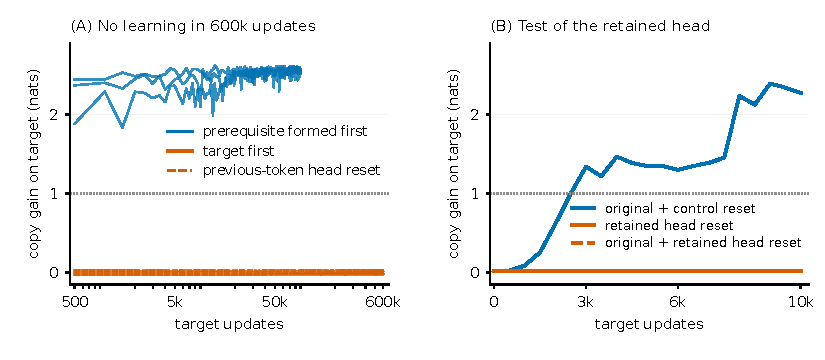
\includegraphics[width=\linewidth]{fig_mechanism.pdf}
\caption{\textbf{Persistent failure and the retained previous-token head.}
(A) Six continuations without the prerequisite (target first and previous-token
reset, three seeds each) stay below 0.03 nats through 600,000 updates; with the
prerequisite, the model learns within 500 updates (logarithmic axis). (B) In the
one model that learned after the previous-token reset, resetting its remaining
previous-token head blocks learning; an equally large control reset does not.}
\label{fig:mechanism}
\end{figure}

For each original seed, the target-first model repeats the warm-up and trains
continuously from target batch zero to 600,000. The previous-token-reset model
restores its archived 90,000-update model and optimizer state, verifies the
data-stream position and trains a further 510,000 updates. We evaluate every 500
updates. A memory fault at launch required restarting from the warm-up and the
archived endpoint, respectively; no outcome informed the restart, and we replace no
seed (Table~\ref{tab:longhorizon}). The 1,200-fold comparison uses learning by 500
updates when the prerequisite is present.

\begin{table}[!htbp]
\centering\small
\caption{Long continuations without the prerequisite. End values average the
last five evaluations.}
\label{tab:longhorizon}
\begin{tabular}{lllllll}\toprule
seed & condition & updates & max copy gain & first $\ge$1 nat & end copy gain & end $d{=}64$ \\
\midrule
531 & target first & 600,000 & 0.00 & none & -0.01 & 0.01 \\
531 & previous-token reset & 600,000 & 0.00 & none & 0.00 & 0.01 \\
532 & target first & 600,000 & 0.03 & none & 0.02 & 0.00 \\
532 & previous-token reset & 600,000 & 0.03 & none & 0.02 & 0.00 \\
533 & target first & 600,000 & -0.02 & none & -0.02 & 0.01 \\
533 & previous-token reset & 600,000 & -0.01 & none & -0.02 & 0.01 \\
\bottomrule\end{tabular}
\end{table}

\section{The retained previous-token head}
\label{app:retained}
For each of the nine models with a previous-token reset, Table~\ref{tab:readiness}
gives the largest mean previous-token attention of any first-layer head immediately
after the reset. We made this measurement after all outcomes were known, so it is
descriptive. In the one model that learned (2642), the head that the selection rule
reset had tied with another head on ablation effect, and the other head has
previous-token attention of 0.981.

We then returned to that model's checkpoint after the circuit formed and, under a
protocol written in advance, reset (i) the retained previous-token head, (ii) both
it and the originally reset head, or (iii) the original head and a low-effect
control head (equal parameter count to ii). Only (iii) learns
(Table~\ref{tab:retained}; \figref{fig:mechanism}B). A thermal abort interrupted the
first attempt; the complete rerun used the same checkpoint, protocol and criteria.

\begin{table}[!htbp]
\centering\small
\caption{All nine models with a previous-token reset: largest previous-token
attention remaining in any first-layer head after the reset.}
\label{tab:readiness}
\begin{tabular}{lllll}\toprule
group & seed & remaining prev.-token attention & updates & first $\ge$1 nat \\
\midrule
original & 531 & 0.148 & 90,000 & none \\
original & 532 & 0.015 & 90,000 & none \\
original & 533 & 0.102 & 90,000 & none \\
fresh & 1541 & 0.011 & 90,000 & none \\
fresh & 1542 & 0.011 & 90,000 & none \\
fresh & 1543 & 0.011 & 90,000 & none \\
broader lesion & 2641 & 0.011 & 10,000 & none \\
broader lesion & 2642 & 0.981 & 10,000 & 3,000 \\
broader lesion & 2643 & 0.011 & 10,000 & none \\
\bottomrule\end{tabular}
\end{table}

\begin{table}[!htbp]
\centering\small
\caption{Targeted resets in model 2642 (10,000 updates).}
\label{tab:retained}
\begin{tabular}{lllll}\toprule
reset & remaining attention & first $\ge$1 nat & end copy gain & end $d{=}64$ \\
\midrule
retained head & 0.015 & none & 0.016 & 0.023 \\
original + retained & 0.011 & none & 0.016 & 0.020 \\
original + control & 0.981 & 3,000 & 2.269 & 0.617 \\
\bottomrule\end{tabular}
\end{table}

\section{Four-layer model}
\label{app:breadth}
We repeat the order comparison in two seeds of a four-layer pre-normalized
transformer with MLP blocks (width 256, eight heads, MLP width 1,024), with the same
formation rule and 60,000-update target blocks. Presenting the target after the
circuit forms yields 2.58/2.55 nats of copy gain and 0.55/0.66 distance-64 accuracy
at the end; presenting it first yields 0.001/0.005 nats and 0.010/0.015.

\section{Pythia-160M: complete results}
\label{app:pythia}

\paragraph{Order and replay.}
The order study starts from Pythia-160M at step 512. Induction training ends after
two consecutive ordinary-induction accuracies of at least 0.70 (minimum 300 updates,
cap 6,000). Target blocks last 500 updates, and we evaluate every 50 updates
(Table~\ref{tab:r3}).

\begin{table}[!htbp]
\centering\small
\caption{Pythia-160M order and replay. $k$ is the induction-training length;
\emph{pre-replay} is target accuracy after induction training but before the target
stream is shown again. Streams 8 and 9 are paired within each run.}
\label{tab:r3}
\resizebox{\linewidth}{!}{%
\begin{tabular}{llrrrrrrrl}\toprule
 & & & \multicolumn{2}{c}{target after induction} & \multicolumn{2}{c}{target first} & \multicolumn{2}{c}{replay} & \\
\cmidrule(lr){4-5}\cmidrule(lr){6-7}\cmidrule(lr){8-9}
run & stream & $k$ & first $\ge0.5$ & end & max & pre-replay & first $\ge0.5$ & end & result\\\midrule
base & 8 & 2,200 & 100 & 1.000 & 0.066 & 0.000 & 100 & 0.996 & pass \\
base & 9 & 2,200 & 100 & 1.000 & 0.039 & 0.000 & 100 & 1.000 & pass \\
seed 1 & 8 & 2,400 & 100 & 0.992 & 0.062 & 0.000 & 100 & 1.000 & pass \\
seed 1 & 9 & 2,400 & 100 & 0.996 & 0.047 & 0.000 & 100 & 0.996 & pass \\
seed 2 & 8 & 2,500 & 100 & 1.000 & 0.043 & 0.000 & 100 & 1.000 & pass \\
seed 2 & 9 & 2,600 & 100 & 1.000 & 0.051 & 0.000 & 100 & 0.996 & pass \\
\bottomrule\end{tabular}}
\end{table}

\paragraph{Training-only suppression.}
At step 1000 of the same three runs, the selection rule (0.2 ceiling) chooses four
heads. Before training, suppressing them lowers induction from at least 0.699 to at
most 0.023, while the controls retain at least 0.699. Each condition starts from the
public checkpoint with a fresh optimizer and consumes 500 batches of the same
stream. A pre-hook zeros the selected head channels before the attention output
projection, only for the six mapped-copy examples in each batch.

Target accuracy under suppression never exceeds 0.047, while every control reaches
at least 0.996 (Table~\ref{tab:r5}). The suppressed models end with lower
(unsuppressed) ordinary induction than the controls (0.22--0.49 against at least
0.74), while their natural-text loss differs by at most 0.024 nats. The
intervention therefore changes how induction itself develops, and we interpret it
as a requirement on the learning trajectory. Evaluated \emph{with} the suppression
applied, the suppressed models also stay below 0.10 (Table~\ref{tab:r6}).

\begin{table}[!htbp]
\centering\small
\caption{Pythia-160M training-only suppression (original three runs). \emph{Induction
probe} is the manipulation check before training. Target columns are maxima over
500 updates, evaluated without suppression.}
\label{tab:r5}
\resizebox{\linewidth}{!}{%
\begin{tabular}{llrrrrrrl}\toprule
 & & \multicolumn{3}{c}{induction probe} & \multicolumn{2}{c}{target maximum} & & \\
\cmidrule(lr){3-5}\cmidrule(lr){6-7}
run & stream & intact & suppressed & control & suppressed & control & control first $\ge0.5$ & result\\\midrule
base & 8 & 0.699 & 0.000 & 0.699 & 0.012 & 1.000 & 200 & pass \\
base & 9 & 0.699 & 0.000 & 0.699 & 0.027 & 0.996 & 200 & pass \\
seed 1 & 8 & 0.734 & 0.023 & 0.730 & 0.016 & 1.000 & 200 & pass \\
seed 1 & 9 & 0.734 & 0.023 & 0.730 & 0.047 & 1.000 & 200 & pass \\
seed 2 & 8 & 0.730 & 0.004 & 0.738 & 0.020 & 1.000 & 200 & pass \\
seed 2 & 9 & 0.730 & 0.004 & 0.738 & 0.020 & 0.996 & 200 & pass \\
\bottomrule\end{tabular}}
\end{table}

\paragraph{Thirteen further pretraining runs.}
We apply the identical protocol to the thirteen remaining public PolyPythias 160M
runs at step 1000: seven with new initialization and data order (seeds 3--9), three
with the original weights and a new data order, and three with the original data
order and new weights. Eligibility requires induction of at least 0.5, suppressed
induction of at most 0.2 with a drop of at least 0.3, control induction of at least
0.5 with a drop of at most 0.15, and initial target accuracy of at most 0.1. All
thirteen runs are eligible, and all pass on both streams
(Table~\ref{tab:polypythia}).

\begin{table}[!htbp]
\centering\small
\caption{The thirteen additional pretraining runs (streams 8/9). Target columns are
maxima over 500 updates. The last two columns evaluate the controls at the end;
\emph{key swap} requires both answers of a pair to be correct.}
\label{tab:polypythia}
\resizebox{\linewidth}{!}{%
\begin{tabular}{llllll}\toprule
run & induction & target: suppressed & target: control & key swap & key deleted \\
\midrule
seed 3 & 0.691 & 0.055/0.055 & 1.000/1.000 & 0.993/0.993 & 0.051/0.039 \\
seed 4 & 0.715 & 0.027/0.023 & 1.000/1.000 & 0.986/0.993 & 0.039/0.031 \\
seed 5 & 0.676 & 0.031/0.047 & 0.996/1.000 & 0.986/0.993 & 0.043/0.047 \\
seed 6 & 0.672 & 0.051/0.066 & 0.996/1.000 & 0.993/0.986 & 0.023/0.043 \\
seed 7 & 0.711 & 0.023/0.027 & 1.000/0.992 & 0.993/0.993 & 0.039/0.023 \\
seed 8 & 0.641 & 0.062/0.059 & 0.996/1.000 & 0.959/0.986 & 0.062/0.047 \\
seed 9 & 0.723 & 0.016/0.020 & 1.000/1.000 & 0.966/1.000 & 0.027/0.070 \\
data 1 & 0.680 & 0.035/0.020 & 0.996/0.996 & 0.986/0.986 & 0.047/0.020 \\
data 2 & 0.664 & 0.008/0.016 & 1.000/1.000 & 0.986/1.000 & 0.051/0.035 \\
data 3 & 0.734 & 0.016/0.020 & 0.996/0.996 & 0.980/0.972 & 0.074/0.043 \\
weight 1 & 0.738 & 0.020/0.031 & 1.000/1.000 & 0.980/0.993 & 0.074/0.047 \\
weight 2 & 0.711 & 0.020/0.020 & 0.996/1.000 & 0.966/1.000 & 0.055/0.047 \\
weight 3 & 0.680 & 0.027/0.031 & 0.996/1.000 & 0.993/0.993 & 0.043/0.051 \\
\bottomrule\end{tabular}}
\end{table}

\begin{table}[!htbp]
\centering\small
\caption{Key dependence and evaluation mode in the six original run--stream pairs. Suppressed
columns are maxima over updates 0--500 with the suppression off or on at
evaluation; control columns are at update 500. Pair counts are 147 (stream 8) and
142 (stream 9).}
\label{tab:r6}
\begin{tabular}{llrrrrr}\toprule
 & & \multicolumn{2}{c}{suppressed, maximum} & \multicolumn{3}{c}{control, endpoint} \\
\cmidrule(lr){3-4}\cmidrule(lr){5-7}
run & stream & off & on & intact & key deleted & key swap \\\midrule
base & 8 & 0.012 & 0.074 & 0.984 & 0.047 & 0.980 \\
base & 9 & 0.027 & 0.051 & 0.996 & 0.035 & 0.993 \\
seed 1 & 8 & 0.016 & 0.098 & 0.992 & 0.043 & 0.993 \\
seed 1 & 9 & 0.047 & 0.094 & 0.996 & 0.043 & 0.986 \\
seed 2 & 8 & 0.020 & 0.062 & 0.996 & 0.055 & 0.986 \\
seed 2 & 9 & 0.020 & 0.051 & 0.988 & 0.039 & 0.965 \\
\bottomrule\end{tabular}
\end{table}

\section{Blocking only the gradient through the prerequisite}
\label{app:gradientblock}
To separate the forward computation of the induction heads from their plasticity,
we keep the heads' forward outputs on target examples but detach them (and their
output-projection columns) from the target loss, so that target examples cannot
send gradient through these paths. Ordinary induction and natural-text examples
update all parameters normally. Four of the six run--stream pairs exceed 0.5
accuracy, but only one passes both key criteria (Table~\ref{tab:gradientblock}).
Some models therefore learn substantially without target gradient through these
heads, and the suppression result in \secref{sec:pythia} depends on removing the
forward computation.

\begin{table}[!htbp]
\centering\small
\caption{Target-gradient blocking with the induction heads' forward computation
kept. All accuracies are measured without the intervention.}
\label{tab:gradientblock}
\begin{tabular}{llllll}\toprule
run & stream & first $\ge0.5$ & end target & key swap & key deleted \\
\midrule
base & 8 & 500 & 0.621 & 0.381 & 0.039 \\
base & 9 & 500 & 0.613 & 0.423 & 0.047 \\
seed 1 & 8 & 450 & 0.680 & 0.483 & 0.020 \\
seed 1 & 9 & 450 & 0.895 & 0.831 & 0.031 \\
seed 2 & 8 & none & 0.039 & 0.000 & 0.051 \\
seed 2 & 9 & none & 0.016 & 0.000 & 0.031 \\
\bottomrule\end{tabular}
\end{table}

\section{Loss-matched controls}
\label{app:lossmatched}
Selection uses only the calibration probes (seed 1701): 256 ordinary induction
sequences and 64 natural-text windows. For every head we measure natural-text loss
and induction accuracy with that head alone zeroed. A head is eligible if its
individual removal keeps induction at 90\% or more of its intact value. We add
eligible heads in decreasing order of their individual loss increase until the set
contains at least as many heads as the circuit and its joint removal increases
natural-text loss at least as much as the circuit's joint removal.

Table~\ref{tab:lossmatched} reports the selections and training outcomes under the
scaling-study protocol ($3\times10^{-5}$, 2,000 updates, streams 38/39).
Individually, induction heads cost little natural-text loss (0.006--0.046 nats each
at 160M), but jointly they cost 0.40 nats, which is why many non-induction heads
are needed to match them.

\begin{table}[!htbp]
\centering\small
\caption{Loss-matched controls. Loss increase and induction are measured with the
set jointly zeroed on the calibration probes. \emph{First learned} uses the full
key-dependent criterion (streams 38/39). $^\ast$From the 10,000-update runs; the
end target for that row is at 10,000 updates.}
\label{tab:lossmatched}
\begin{tabular}{lcccccc}\toprule
model & set & heads & loss increase (nats) & induction & first learned & end target \\
\midrule
160M & none & 0 & --- & 0.70 & 350 / 350 & 1.00 / 1.00 \\
160M & induction & 4 & 0.40 & 0.00 & 6,400 / 6,300$^\ast$ & 0.99 / 1.00 \\
160M & loss-matched & 16 & 0.43 & 0.66 & 350 / 400 & 1.00 / 1.00 \\
410M & none & 0 & --- & 0.61 & 150 / 150 & 1.00 / 1.00 \\
410M & induction & 8 & 0.23 & 0.01 & 900 / 900 & 1.00 / 1.00 \\
410M & loss-matched & 8 & 0.27 & 0.61 & 150 / 200 & 1.00 / 1.00 \\
\bottomrule\end{tabular}
\end{table}

\section{Scaling study: details and complete results}
\label{app:scaling}

\begin{table}[!htbp]
\centering\small
\caption{Models and selected interventions. Holdout values are ordinary induction
accuracy on a 1,024-example probe used only after selection (intact / circuit
suppressed / control suppressed).}
\label{tab:selection}
\begin{tabular}{llcccl}\toprule
model & step & layers $\times$ heads & head dim & suppressed & holdout \\
\midrule
160M & 1000 & 12 $\times$ 12 & 64 & 4 & 0.772 / 0.004 / 0.786 \\
410M & 1000 & 24 $\times$ 16 & 64 & 8 & 0.627 / 0.006 / 0.664 \\
1B & 1000 & 16 $\times$ 8 & 256 & 8 & 0.803 / 0.003 / 0.712 \\
1.4B & 1000 & 24 $\times$ 16 & 128 & 7 & 0.821 / 0.017 / 0.833 \\
2.8B & 1000 & 32 $\times$ 32 & 80 & 4 & 0.711 / 0.004 / 0.715 \\
6.9B & 2000 & 32 $\times$ 32 & 128 & 24 & 0.700 / 0.017 / 0.594 \\
12B & 2000 & 36 $\times$ 40 & 128 & 32 & 0.793 / 0.006 / 0.793 \\
\bottomrule\end{tabular}
\end{table}

\paragraph{Eligibility.}
At step 1000, 6.9B and 12B do not meet the pre-specified requirement that
unsuppressed induction be at least 0.5 on both calibration probes (0.37/0.39 and
0.50/0.48), so we do not train them at step 1000. A separately specified search
selected step 2000 for both. We trained 6.9B; we did not train 12B, for lack of
storage. The number of heads needed for near-complete suppression is not monotonic
in size, and head counts are not comparable across architectures, because head
width and count differ.

\paragraph{Head count.}
The delay depends on how completely induction is suppressed at the start. On fresh
streams 38/39 at 410M with the original training labels, suppressing four heads
(leaving 6--8\% induction) permits key-dependent learning by update 400/450 (end
accuracy 0.95/0.98), while eight heads (0.6\%) block it at 500 updates
(0.004/0.004). With corrected labels the four-head runs also learn within 500
updates (0.96/0.98), and the eight-head runs learn at update 900.

At 1.4B, four heads permit learning by update 350 (end accuracy 0.95/0.99), and
seven give partial learning that fails the key test (0.20/0.14 accuracy, key swap
0.02/0.01). At 1B on streams 78/79, four heads permit learning (0.99/0.93) with
masked induction recovering to 0.73--0.82, and eight heads block it (0.00/0.00). In
every case the controls learn.

\paragraph{Independent 410M pretraining runs.}
In three further public 410M runs (step 1000; 8, 4 and 4 heads selected), the
suppressed models stay at 0.00--0.02 target accuracy through 500 updates on both
streams, with masked induction at or below 0.004, and all twelve controls learn.
Over 2,000 updates (Table~\ref{tab:replicates}), run 1 (eight heads suppressed)
learns at update 900 on both streams, like the reference run. Runs 2 and 3 (four
heads each) stay blocked on both streams: target accuracy never exceeds 0.10 and
0.004, and masked induction never exceeds 0.004.

The three runs leave 8, 3 and 3 unsuppressed heads with induction attention of at
least 0.2 (strongest 0.45, 0.48 and 0.28). We computed these counts while run 2 was
in progress and before run 3 began, and predicted that run 3 would learn later than
run 1.

\begin{table}[!htbp]
\centering\small
\caption{Independent 410M pretraining runs over 2,000 updates (stream 38 / 39).
\emph{Masked induction $>0.2$} is the first evaluation at which ordinary induction
with the suppression mask applied exceeds 0.2.}
\label{tab:replicates}
\begin{tabular}{lccccc}\toprule
run & heads & first learned & masked induction $>0.2$ & end target & end masked induction \\\midrule
\inputrows{generated/tab_replicates.tex}
\bottomrule\end{tabular}
\end{table}

\paragraph{Corrected induction examples.}
Correcting the ordinary induction training rows (\appref{app:pythiamethods})
preserves every qualitative outcome at 160M (4 heads), 410M (4 and 8 heads) and 1B
(8 heads) on both streams: the suppressed models' target accuracy is 0/0,
0.96/0.98, 0.04/0.02 and 0/0, respectively, and the controls learn.

\paragraph{2,000-update runs.}
Table~\ref{tab:horizon} gives endpoints of the 2,000-update runs. The first 500
updates of each run reproduce the earlier 500-update runs exactly.

\begin{table}[!htbp]
\centering\small
\caption{2,000-update endpoints (streams 38/39 for 160M and 410M; 78/79 for 1B).
\emph{Masked induction} applies the original suppression mask at evaluation.}
\label{tab:horizon}
\begin{tabular}{llcccc}\toprule
model & condition & target & key swap & key deleted & masked induction \\
\midrule
160M & suppressed & 0.000 / 0.000 & 0.000 / 0.000 & 0.023 / 0.023 & 0.000 / 0.000 \\
160M & control & 1.000 / 1.000 & 1.000 / 1.000 & 0.047 / 0.031 & --- \\
410M & suppressed & 0.996 / 0.996 & 0.993 / 0.993 & 0.004 / 0.004 & 0.883 / 0.816 \\
410M & control & 0.996 / 1.000 & 1.000 / 1.000 & 0.020 / 0.008 & --- \\
1B & suppressed & 0.988 / 0.984 & 0.984 / 0.987 & 0.000 / 0.000 & 0.891 / 0.965 \\
1B & control & 1.000 / 1.000 & 1.000 / 1.000 & 0.000 / 0.000 & --- \\
\bottomrule\end{tabular}
\end{table}

\paragraph{Longer training at 160M and 2.8B.}
We continue the 160M suppressed runs to 10,000 updates (evaluated every 100) and
the 2.8B suppressed runs to 2,000 updates, on the same corrected streams 38/39,
whose first 2,000 batches are byte-identical to those of the 2,000-update runs.
Table~\ref{tab:newruns} gives their outcomes. Both 160M runs first learn at 6,400
and 6,300 updates. In both, target accuracy passes 0.1 at updates 3,800--4,000,
while masked induction first exceeds 0.02 only at 5,100--5,300. We did not rerun
the 2.8B controls on these streams; controls on the 500-update streams learned by
update 150--200.

\paragraph{Which heads carry the rebuilt circuit at 6.9B.}
With the original 24 heads suppressed, we rank the remaining heads of each 6.9B
model that learned by induction attention on fresh probes and add heads until
induction falls to at most 0.02. Twelve (stream 58) or eleven (stream 59) additional
heads suffice, verified on a 1,024-example holdout (induction to 0.01--0.02).
Adding them lowers target accuracy from 1.00 to 0.28/0.32 and key-swap accuracy to
0.13/0.09, while layer-matched controls leave target accuracy at 1.00/0.97. The
additional heads cost 0.09/0.05 nats of natural-text loss relative to the controls.
In the pretrained 6.9B model the same 36 heads remove induction entirely, so this
analysis cannot tell whether they were capable of induction beforehand.

\paragraph{Distance coverage.}
Induction probes at distances 24, 44, 64 and 96, in native and position-matched
versions, show the same pattern. The trained 160M suppressed models score zero with
the mask applied at every distance. The 410M and 1B suppressed models recover masked
induction at all distances, including 96, which lies outside the training range
(recovery there is weaker). The fixed 24-head mask at 6.9B leaves under 1.8\%
induction initially across all eight probes, and 66--92\% after training.

\section{Adaptive suppression}
\label{app:adaptive}
Both adaptive procedures start from the fixed 8-head 410M intervention and use the
2,000-update streams 38/39. Every 50 updates, after evaluation, the procedure
computes a score with the current mask applied. If the score exceeds the
threshold, the procedure repeatedly adds the two unsuppressed heads with the highest
query-to-source attention (under the current mask) until the score is back at or
below the threshold.

\emph{Induction-triggered} suppression uses ordinary induction accuracy on the two
calibration probes as the score (threshold 0.02, the selection criterion).
\emph{Key-triggered} suppression uses the key-swap pass rate on two held-out
mapped-copy probes, generated with the stream's mapping but disjoint from the
evaluation probes (threshold 0.10). This score responds only to key-dependent
retrieval of the target, not to shortcuts.

A \emph{yoked control} replays the key-triggered schedule of additions (same
updates, same layers, same counts) but adds the lowest-attention heads in those
layers. Because the yoked controls learn before the first addition, we also run a
\emph{static control} that masks, from update 0, as many layer-matched
lowest-attention heads (attention at most 0.013) as the key-triggered runs end with
(22 and 16). Until the first addition, the adaptive runs reproduce the fixed-mask
runs exactly (checked at every evaluation).

Table~\ref{tab:newruns} reports these runs together with the other follow-up
experiments.

\begin{table}[!htbp]
\centering\small
\caption{All follow-up runs (streams 38/39; learning rate $3\times10^{-5}$; values are
stream 38 / stream 39). \emph{Heads} is the number of suppressed heads at the end.
\emph{First learned} uses the full key-dependent criterion, evaluated every 50
updates (every 100 for the 10,000-update runs). \emph{Masked induction} is ordinary
induction at the end with the run's final mask applied.}
\label{tab:newruns}
\setlength{\tabcolsep}{3pt}
\resizebox{\linewidth}{!}{%
\begin{tabular}{lcccccc}\toprule
condition & heads & updates & first learned & end target & end key swap & masked induction \\\midrule
\inputrows{generated/tab_new_runs.tex}
\bottomrule\end{tabular}}
\end{table}

\section{Which heads carry the rebuilt circuit at 410M and 1B}
\label{app:regrowth}
For each 2,000-update endpoint we measure, with the original mask applied, every
head's query-to-source attention on the two calibration probes. We then mask the
top-$k$ remaining heads in addition to the original set ($k\in\{2,4,8,16\}$), or
$k$ layer-matched low-attention heads, and measure induction on a held-out probe
(seed 4701, never used for ranking), target accuracy and the key tests.

Table~\ref{tab:regrowthrank} lists, for each endpoint, the four unsuppressed heads
with the highest attention after training, their rank by attention in the
pretrained model (unsuppressed, calibration probes), and their attention before and
after training. The same heads top the list in every condition, and they are ranks
9--13 in the pretrained model, immediately below the suppressed set. Their
attention grows in every condition, but only suppressed training makes them
produce induction when the original heads are masked (last column).
Table~\ref{tab:regrowthabl} gives the ablation results.

We designed this analysis after seeing that the suppressed models learn. The
ranking uses the endpoint attention, and the rank comparison is descriptive. The
prospective test in \secref{sec:scaling} fixes the mask from pretrained attention
alone.

\begin{table}[!htbp]
\centering\scriptsize
\caption{The heads that carry induction after training, with the original mask
applied. \emph{Rank} is the head's rank by induction attention in the pretrained
model (the suppressed heads are ranks 1--8). Attention before and after training
is measured with the original heads masked. \emph{Masked induction} is held-out
induction accuracy with the original suppressed heads zeroed.}
\label{tab:regrowthrank}
\setlength{\tabcolsep}{3pt}
\begin{tabular}{lllllllr}\toprule
model & stream & training & top heads after training & rank & attention before & attention after & masked induction \\\midrule
\inputrows{generated/tab_regrowth_rank.tex}
\bottomrule\end{tabular}
\end{table}

\begin{table}[!htbp]
\centering\small
\caption{Masking the rebuilt heads in suppressed-trained endpoints, in addition to
the original set. Each cell gives rebuilt / layer-matched low-attention heads.}
\label{tab:regrowthabl}
\begin{tabular}{llclll}\toprule
model & stream & added & held-out induction & target & key swap \\\midrule
\inputrows{generated/tab_regrowth_ablation.tex}
\bottomrule\end{tabular}
\end{table}

\paragraph{Backup heads across models.}
Table~\ref{tab:capacity} counts, in each pretrained model, the heads outside the
selected suppression set that attend from the repeated key to its source. Every
model has some. Ordered by the count of heads at or above 0.2 attention, the
suppressed models learn roughly as follows. With one such head (160M), learning
takes 6,300--6,400 updates; with two (1B), 1,200--1,400; with three (160M with only
two heads suppressed), 1,100--1,300, whereas independent 410M runs 2 and 3, also
with three, do not learn within 2,000; and with five to eight (410M reference and
run 1, 2.8B), about 900.

We computed the count for 160M, 410M, 1B, 1.4B and 2.8B after observing that the
suppressed models learn (except at 2.8B, whose long runs came later), and for the
independent 410M runs while run 2 was in progress and before run 3 began. The
relation is only roughly monotone and is confounded by architecture, head width and
checkpoint, so we treat it as suggestive.

\begin{table}[!htbp]
\centering\small
\caption{Backup heads in the pretrained checkpoints (step 1000). Attention
is measured without suppression on the calibration probes; induction accuracy on a
held-out probe, without and with the selected heads suppressed.}
\label{tab:capacity}
\begin{tabular}{lrrrrrrr}\toprule
 & heads & suppressed & \multicolumn{2}{c}{induction} & \multicolumn{2}{c}{other heads with attention} & max other \\
\cmidrule(lr){4-5}\cmidrule(lr){6-7}
model & total & & intact & suppressed & $\ge0.1$ & $\ge0.2$ & attention \\\midrule
\inputrows{generated/tab_capacity.tex}
\bottomrule\end{tabular}
\end{table}

\section{Freezing the lower half of Pythia-1B}
\label{app:prefix}
Starting from Pythia-1B at step 1000, we freeze the embeddings and blocks 0--7 (half
of the 1.01B parameters), which contain the eight selected heads (blocks 4--7). On
target examples, we either remove the heads' contributions or replace them with the
exact contributions of the frozen original (restoration). Ordinary induction and
natural-text examples keep the original computation. Everything else follows the
scaling protocol (learning rate $3\times10^{-5}$, streams 78/79).

Table~\ref{tab:prefix} gives the outcomes. We extended the removal runs from 2,000
to 6,000 updates after partial learning appeared at 2,000; the controls ran for
2,000 updates. Restoration reproduces the trajectories of the intact runs exactly.

The removal-trained models pass the key tests only when evaluated with the heads
still removed. Their ordinary induction under removal stays at or below 2/256 on
our probe. This does not show that the workaround uses no retrieval: it may use
computations that our ordinary-induction probe does not measure. We therefore
describe it as a key-dependent workaround built in the trainable upper layers, not
as learning without the prerequisite.

\begin{table}[!htbp]
\centering\small
\caption{Pythia-1B with the lower half frozen. \emph{Removal on} evaluates the
model with the heads still removed; \emph{native} evaluates it with the original
heads.}
\label{tab:prefix}
\begin{tabular}{lcccc}\toprule
condition (streams 78/79) & first learned & updates & end target & end key swap \\
\midrule
restoration, native & 300 / 300 & 2,000 & 0.984 / 0.980 & 0.992 / 0.973 \\
removal, removal on & 2,750 / 2,800 & 6,000 & 0.980 / 0.980 & 0.945 / 0.960 \\
removal, native & never & 6,000 & 0.023 / 0.039 & 0.000 / 0.000 \\
\bottomrule\end{tabular}
\end{table}

\section{Removing attention to the key}
\label{app:edges}
This intervention is stronger in kind and weaker in interpretation than head
suppression, so we report it separately. On mapped-copy training examples only, it
blocks, in every layer and head, attention from the source marker and every later
position to the four tokens of the earlier key occurrence. Attention to the source
marker itself and to the second key occurrence remains. The control applies the
same cut to the nearest irrelevant four-token block. Ordinary induction and
natural-text examples are unaffected, and evaluation is unmasked.

With learning rate $3\times10^{-5}$ over 2,000 updates, the cut blocks key-dependent
learning at 160M, 410M, 1B and 1.4B on both streams. It never meets the
key-dependence criterion at any of the 41 evaluations, while every intact and
control run learns by update 150--350. At 410M this holds even though the models
learn by update 900 under the fixed eight-head suppression on the same streams.

We do not treat this as evidence about prerequisite circuits, for two reasons.
First, the cut removes information the target needs, namely the earlier key, rather
than a learned computation, so blocking is close to guaranteed unless some circuit
reads the key indirectly. Second, the cut sits at the answer's key, so the pattern
of blocked positions itself reveals where the source is. A model given the mask
geometry and the mapping could solve the task without reading the key, and it would
fail the key-deletion test.

The models trained with the cut do improve their target likelihood without learning
the task. Most of this improvement comes from avoiding the source marker's unmapped
identity (4.6--5.9 nats), with a smaller preference for the correct marker
(1.2--1.6 nats). A restoration experiment at 410M finds that most of this benefit
carries over to a new mapping, which suggests that the models trained with the cut
learn mostly mapping-independent marker statistics.

\section{Additional seeds of the two-layer model}
\label{app:newseeds}
To add seeds to the suppression and supply experiments, we train five new models
(seeds 3541--3545) from scratch with the original warm-up, formation rule, head
selection rule and control-head rule. We then run the unsuppressed,
control-suppressed, suppressed, correct-supply, no-supply and wrong-supply
conditions on the same 1,000 target batches, with the original exact-restoration
checks (frozen weights unchanged, restored computation bit-identical at every
evaluation). All five models form the circuit, and in each the largest-effect head
is a first-layer head.

Table~\ref{tab:newseeds} gives every endpoint. Suppression blocks learning in all
five, and supplying the intact activation restores it to the unsuppressed value.
The unsuppressed copy gain varies more across these models (1.25--2.51 nats) than
across the original three. In one model (3545) the control-head set removes more
short-range accuracy than the original floor would allow (0.49 against 0.60); the
original code records but does not select on this check, and we report the model
unchanged. In none of the new models does replay with both heads enabled reach
1 nat within 1,000 updates after suppressed exposure (maximum 0.30), which is
consistent with the mixed replay outcomes in Table~\ref{tab:stable}.

These runs used a different GPU and library version from the originals. Retraining
seed 531 from scratch reproduces its inputs bit-for-bit and the qualitative
pattern, but not its exact published values, because floating-point differences
change the model in which the circuit forms.

\begin{table}[!htbp]\centering\scriptsize
\caption{Five additional seeds of the two-layer model: copy gain (nats) / distance-64
accuracy after 1,000 target updates. \emph{Replay} is copy gain after 1,000 further
updates of replay with both heads enabled, following suppressed exposure.}
\label{tab:newseeds}
\setlength{\tabcolsep}{2.5pt}
\resizebox{\linewidth}{!}{%
\begin{tabular}{lcccccccccc}\toprule
seed & formed at & head & unsuppressed & control & suppressed & correct supply & no supply & wrong supply & replay \\\midrule
\inputrows{generated/tab_newseeds.tex}
\bottomrule\end{tabular}}
\end{table}

\section{Further experiments}
\label{app:future}
\paragraph{Finer interventions.} Head-level suppression removes everything a head
computes. Suppressing induction at the level of attention edges between specific
positions, QK features \citep{kamath2025tracing} or learned subspaces, with
circuits found by attribution methods such as EAP-IG or edge pruning
\citep{hanna2024faith,bhaskar2024edge} and validated by activation patching
\citep{zhang2024patching}, would show whether the model also routes around a
narrower cut, and would reduce collateral effects. The key-triggered adaptive
procedure in \secref{sec:scaling} is a coarse version of such computation-level
suppression.

\paragraph{Predicting when data will teach.} The rebuilt heads are identifiable
before training by their induction attention. A score built from these backup
heads (for instance, the attention and copying scores of unused heads)
could predict whether and how quickly a model will learn from a given data stream,
and could guide data scheduling. Testing such a predictor prospectively across
PolyPythias runs and checkpoints is a direct next step.

\paragraph{Controlled scaling.} Pythia sizes differ in depth, width, head width and
the maturity of a checkpoint at a given step. Training small families that differ
only in heads per layer or width, forming the same prerequisite and applying the
same computation-level suppression would test whether the delay falls with the
number of candidate backup heads, as our backup-head account predicts. The
escape-dimension view of overparameterization (a preprint;
\citealp{martinelli2026escape}) would suggest a similar dependence on width through
a different mechanism. Such families would also allow direct measurement of the
loss landscape during the delay (for example, the plateau and the curvature along
the parameters of the rebuilt heads).

\paragraph{Suppressing the previous-token step in pretrained models.} In the
two-layer model the previous-token step cannot be rebuilt, while the induction step
can. Our interventions in pretrained models suppress the induction heads.
Suppressing previous-token heads on target examples in Pythia would test whether
the previous-token step is also harder to rebuild at scale.

\paragraph{Other prerequisite families.} Candidate pairs include entity binding as a
prerequisite for multi-hop retrieval, successor or carry circuits for multi-digit
arithmetic, and syntactic heads for agreement. Each admits the same fixed-data
design: training-only suppression, supplying the suppressed output and replay.

\paragraph{Natural pretraining.} The Pythia suite's public data order makes it
possible to intervene on circuits during pretraining itself and ask which later
capabilities are delayed, rather than using synthetic fine-tuning targets.

\paragraph{Robust capability removal.} In larger models, suppressing a prerequisite
delays but does not prevent learning. Whether adaptive, computation-level
suppression can keep a capability from being learned, and at what cost to other
capabilities, bears directly on tamper-resistant unlearning
\citep{tamirisa2025tamper,che2025tampering}.

